\documentclass[11pt]{article}
\usepackage[T1]{fontenc}
\usepackage[utf8]{inputenc}
\usepackage{lmodern}
\usepackage[margin=1in]{geometry}
\usepackage{amsmath,amssymb,amsthm,mathtools}
\usepackage{microtype}
\usepackage{enumitem}
\usepackage{tikz}
\usetikzlibrary{arrows.meta,positioning,calc,decorations.pathreplacing}
\usepackage[numbers,sort&compress]{natbib}
\usepackage[colorlinks=true,linkcolor=blue!45!black,citecolor=blue!45!black,urlcolor=blue!45!black]{hyperref}
\usepackage{bookmark}
\hypersetup{pdftitle={The sharp factor-of-IID threshold for the free Ising model on regular trees},pdfauthor={OpenAI}}
\newtheorem{theorem}{Theorem}[section]
\newtheorem{lemma}[theorem]{Lemma}
\newtheorem{proposition}[theorem]{Proposition}
\newtheorem{corollary}[theorem]{Corollary}
\theoremstyle{definition}
\newtheorem{definition}[theorem]{Definition}
\theoremstyle{remark}
\newtheorem{remark}[theorem]{Remark}
\newcommand{\E}{\mathbb E}
\renewcommand{\P}{\mathbb P}
\DeclareMathOperator{\Var}{Var}
\DeclareMathOperator{\Cov}{Cov}
\DeclareMathOperator{\Aut}{Aut}
\DeclareMathOperator{\dist}{dist}
\newcommand{\dd}{\,\mathrm d}
\newcommand{\1}{\mathbf 1}
\numberwithin{equation}{section}
\setlist{topsep=5pt,itemsep=3pt}
\setlength{\emergencystretch}{2em}
\title{The sharp factor-of-IID threshold\\for the free Ising model on regular trees}
\author{OpenAI}
\date{September 26, 2026}
\begin{document}
\maketitle
\begin{abstract}
For every integer \(d\ge3\) and inverse temperature \(\beta\ge0\), the free
zero-field ferromagnetic Ising measure on the infinite \(d\)-regular tree is
a factor of IID exactly when \(\tanh\beta\le(d-1)^{-1/2}\). We prove the
positive implication, including equality, resolving the conjecture of Nam,
Sly and Zhang; the strict converse is known. The spin factor can be chosen
to commute with every tree automorphism on every label input.
\end{abstract}
\section{Introduction}\label{sec:introduction}

Can the free Ising state on a regular tree be generated from independent
vertex labels without choosing a root? The broadcast description of the
state begins at a vertex and propagates a random spin along the edges.
Its law does not depend on that vertex. A factor construction must also
remove the distinguished vertex from the rule that generates the spins.

Let $T_d=(\mathcal V,\mathcal E)$ be the infinite $d$-regular tree,
$d\ge3$, and put $b=d-1$ and $\theta=\tanh\beta$ for $\beta\ge0$.
The free zero-field Ising law $\mu_{d,\beta}$ is obtained by choosing a
fair spin at one vertex and, independently along edges directed away
from it, letting a child agree with its parent with probability
$(1+\theta)/2$. Its marginal on any finite connected subtree $D$ is
\[
 \mu_{d,\beta}(\sigma|_D=\eta)
   =\frac12\prod_{\{u,v\}\in\mathcal E(D)}
                      \frac{1+\theta\eta_u\eta_v}{2}.
\]
This expression also verifies that the law is invariant under all tree
automorphisms and independent of the chosen broadcast root.

We call a spin law a \emph{factor of IID} if it is the law of
$\Phi(U)$ for independent uniform labels $(U_v)_{v\in\mathcal V}$ and
a measurable map $\Phi:[0,1]^{\mathcal V}\to\{-1,1\}^{\mathcal V}$
satisfying
\begin{equation}\label{eq:equivariance}
 \Phi(gU)=g\Phi(U)\quad\text{almost surely for each fixed }
                 g\in\Aut(T_d),\qquad (gx)_v=x_{g^{-1}v}.
\end{equation}
The exceptional null set may depend on $g$. For spin laws this convention
is equivalent to requiring a Borel factor equivariant on every input:
Lemma~\ref{lem:pointwise-spin-factor} constructs such a version.
The input contains no distinguished root or end. Measurability does not require a spin to be
determined by finitely many labels; no finitary coding or coding-radius
estimate is asserted.

\begin{theorem}\label{thm:main}\label{thm:sharp}
For every integer $d\ge3$ and every $\beta\ge0$, the free zero-field
Ising law $\mu_{d,\beta}$ is a factor of IID in the sense of
\eqref{eq:equivariance} if and only if
\[
                         \tanh\beta\le(d-1)^{-1/2}.
\]
In this range the factor can be chosen to commute with every
automorphism on every label input.
\end{theorem}

The construction proves the positive implication, including equality.
The strict converse is known: the obstruction beyond the reconstruction
threshold is due to Sly, as recorded and proved in
Lyons~\cite[Section~3 and Corollary~3.2]{Lyons}. We use the quantitative correlation bound
of Backhausz, Szegedy and Vir\'ag~\cite[Theorem~3.1 in
arXiv:1305.6784v1]{BSV} to give that implication below.
The map is obtained for each fixed $d$ and $\beta$ in the permitted
range; no parameter-uniform or computational bound is asserted.

For the free state on $T_d$, reconstruction from distant levels is
possible exactly when $b\theta^2>1$; equivalently, the free Gibbs state
is extremal exactly when $b\theta^2\le1$. For the regular-tree result,
including equality, see the Bethe-lattice work of Bleher, Ruiz, and
Zagrebnov~\cite{BleherRuizZagrebnov1995} and
Ioffe~\cite{Ioffe1996Bethe}. Ioffe~\cite{Ioffe1996GeneralTrees} and
Evans, Kenyon, Peres, and Schulman~\cite{EvansKenyonPeresSchulman2000}
developed branching-number criteria on general trees away from equality.
Pemantle and Peres~\cite[Theorem~2.1]{PemantlePeres} later gave an
electrical-capacity criterion for free-state extremality for couplings
bounded above and away from zero, which also covers critical cases.

Reconstruction asks whether distant spins retain information about a
fixed spin. The factor question asks for a rule that generates the
entire law from independent labels. Nonreconstruction supplies no such
rule, and a weak limit of factor laws need not itself be a factor
\cite[Corollary~3.3]{Lyons}. Thus equality requires a construction that retains
measurable dependence on its independent input.

In the uniqueness range $\theta\le b^{-1}$, including equality, a
finite-cluster construction gives the factor; see
Lyons~\cite[Section~3]{Lyons}. Nam, Sly and
Zhang~\cite[Theorem~1 and Section~2.2 in arXiv:2012.09484v2]{NSZ}
used posterior-drift stochastic differential equations driven by IID
Brownian motions to construct the free Ising law as a factor for
$d\ge d_0$ and $\theta\le c/\sqrt{d-1}$, for unspecified absolute
constants $c,d_0>0$. Their construction takes root-independent limits
of finite-volume solutions.
Theorem~\ref{thm:main} proves their conjecture for every $d\ge3$,
including equality and their pointwise convention for equivariance.

\paragraph{The known converse.}
For a centered variance-one real vertex factor, the BSV bound is
\[
 |\E[Z_oZ_v]|\le
       \left(1+\frac{d-2}{d}n\right)b^{-n/2},
                  \qquad \dist(o,v)=n.
\]
It applies also under~\eqref{eq:equivariance}. To check this,
condition the observable at $o$ on the labels in its radius-$R$ ball
and average a Borel version over the finite automorphism group of that
rooted ball. Every such permutation extends to a tree automorphism
fixing $o$, so uniqueness of conditional expectation leaves this
average unchanged almost surely. It now defines an exactly invariant
local rule. Apply the same rule at every vertex. These local factors
converge in $L^2$ at each vertex to the original factor, because the
balls exhaust the label coordinates. For all sufficiently large $R$
their variances are positive. Center and normalize them, apply BSV,
and pass to the limit in variances and covariances on this same IID
probability space. Since the Ising spins have mean zero, variance one
and correlation $\theta^n$, the bound would require
$(\theta\sqrt b)^n\le1+(d-2)n/d$. This is impossible when
$\theta>b^{-1/2}$.

\subsection{Why independent innovations determine the spins}

We follow the observation framework of Nam--Sly--Zhang. On an auxiliary
probability space, sample the desired spin configuration $\sigma$ and
independent standard Brownian motions $B_v$, and observe
\[
 X_v(t)=t\sigma_v+B_v(t),\qquad
 m_v(t)=\E[\sigma_v\mid X_u(s):u\in\mathcal V,\ 0\le s\le t].
\]
The finite-dimensional posterior evolution also belongs to stochastic
localization. Eldan~\cite{Eldan2013} developed the underlying localization
scheme, and El Alaoui and Montanari~\cite[Section~3, Theorem~2]{ElAlaouiMontanari2022}
give the fixed-covariance Gaussian-observation formulation used here.
Subtracting the conditional drift gives
\[
                      W_v(t)=X_v(t)-\int_0^t m_v(s)\,ds.
\]
These innovations are independent Brownian motions in the observation
filtration. This property alone does not make $X$ a function of $W$:
the original construction still used the spins. Classical innovations
theory separates the Brownian property from generation of the
observation filtration~\cite[Lemma~2.2 and Remark~2.2]{FujisakiKallianpurKunita1972}.
Proving that the innovations determine $X$ is the central step here.

A companion construction for the free uniform spanning forest uses a
uniform Lipschitz response bound in the coordinate supremum norm to
invert the innovations causally for every continuous input
\cite[Section~4]{OpenAIFUSF2026}.
Here recovery instead follows from equality of conditional copies under
the observation law.

Take two observations $X,X'$ independently conditional on the entire
innovation array $W$. They have the same marginal law and share the
same innovations. Conditioning on the full paths could in principle
expose their future increments through an observation past. We prove
that it does not: the conditional law of either observation past given
all of $W$ depends only on the past of $W$. Hence $W$ remains Brownian
in the joined filtration, and the equations for both observations use
the same driving Brownian motions. This is the compatibility principle
for conditional copies~\cite[Lemmas~2.11--2.12 in arXiv:1305.6747v2]{Kurtz2014};
we prove the required statement
and the transport of the stochastic integrals directly.

We then show that these particular copies agree. For each coordinate,
conditional independence gives
\[
 \E[(X_v(t)-X'_v(t))^2\mid W]
                  =2\Var(X_v(t)\mid W).
\]
Equality therefore forces the conditional law of $X$ given
$W$ to be a point mass. Finally
\[
                         \frac{X_v(n)}n\longrightarrow\sigma_v
                           \quad\text{almost surely}
\]
recovers the spins from $W$. A common measurable sampler converts one
uniform label at each vertex into its Brownian path. This gives a spin
factor satisfying~\eqref{eq:equivariance}; finite-ball averaging then
selects an everywhere equivariant version with the same law.

\subsection{What changes at the critical point}

The tree gives a concrete equation for comparing the copies. Set
$h_v=\operatorname{atanh}m_v$. If $T_{j\to i}$ is the component containing
$j$ after deleting $ij$, define its field by
\[
 h_{j\to i}(t)=\operatorname{atanh}
   \E[\sigma_j\mid X_u(s):u\in T_{j\to i},\ 0\le s\le t],
\]
using the unconditional prior on that component.
For a path $v=v_0,\ldots,v_r=u$, the field-response
coefficient is
\[
 c_{vu}=\theta^r\prod_{i=1}^r a(h_{v_i\to v_{i-1}}),
 \qquad
 a(z)=\frac{1-\tanh^2z}{1-\theta^2\tanh^2z},\qquad c_{vv}=1.
\]
The innovation equation is
\[
 dh_v=\sum_u c_{vu}\,dW_u+m_v A_v\,dt,
                  \qquad A_v=\sum_u c_{vu}^2.
\]
Its infinite sum requires proof. At criticality we obtain
$\E A_v(t)\le C/\min(\sqrt t,1)$ for $t>0$, so the row is integrable
down to time zero. An exact covariance-energy identity and a testing
argument establish the equation without a residual martingale.

For the conditional copies, let
$V(t)=\E[(h_o(t)-h'_o(t))^2]$; invariance makes the choice of $o$
irrelevant. It starts at zero. Below the threshold, the squared factor
$\theta^{2r}$ and the shell size $d b^{r-1}$ give a summable geometric
series, yielding $V'\le CV$ and thus equality of the copies.
At $b\theta^2=1$ those two factors cancel exactly.

Three estimates replace the lost geometric decay. First, an intact side
branch attenuates a path product on the length scale $t^{-1/2}$ at small
times. Second, spatial cancellation bounds the variance of a sum of
differences between the two copies' $\log a(h_{j\to i})$ factors by
the path length times the variance at one edge. The spectral
bound is proved for differences $f(X)-f(X')$, with the same
square-integrable equivariant vertex observable $f$ applied to each copy, and their closed
linear span. No spectral bound for every function of the pair is assumed.
The operator argument is related to the correlation methods of
Backhausz--Szegedy--Vir\'ag~\cite{BSV} and
Backhausz--Gerencs\'er--Harangi--Vizer~\cite{BGHV}.
Third, concentration of path averages makes the attenuation
usable with discrepancy weights that depend on the same observations.
Both path orientations are needed in this averaging argument.

These estimates leave one small-time difficulty: the leading noise
term is of order $S(t)/t$, where
\[
 S(t)=\E\Bigl[\bigl(\log a(h_{j\to i}(t))
                    -\log a(h'_{j\to i}(t))\bigr)^2\Bigr].
\]
The elementary bound $S\le CV$ would leave a nonintegrable coefficient.
We prove instead a small-field tail estimate and use the vanishing
derivative of $\log a$ at zero to improve that comparison. The complete
noise and drift calculation then gives an integrable Osgood-type
inequality for $V$, forcing $V=0$. The moment estimate is proved beside
this final comparison, where its purpose becomes explicit.

\paragraph{Notation and organization.}
The case $\theta=0$ is already IID, so the proof below assumes
$0<\theta\le b^{-1/2}$. Constants $c,C>0$ may depend on the fixed
$d,\theta$ and may change between occurrences; a subscript $T$ permits
additional dependence on a fixed finite time horizon. Every path is
simple unless specified otherwise, and all logarithms are natural.
Roots used to describe subtrees or compute norms are auxiliary choices
in the proof, not inputs to the factor.

Sections~\ref{sec:observations}--\ref{sec:innovations} develop the
posterior identities, critical information bounds, and infinite
innovation equation. Section~\ref{sec:coupling} constructs the conditional
copies and proves their equality below the threshold.
Sections~\ref{sec:spectrum} and~\ref{sec:path-averages} establish spatial
cancellation and concentration of path averages.
Section~\ref{sec:uniqueness-factor} proves the small-field tail estimate,
completes the critical comparison, and recovers the factor from the
innovations.

\section{Posterior fields along the tree}
\label{sec:observations}

The observation construction reduces the factor problem to a question
about conditional spin laws.  We first describe those laws on a finite
subtree, where the Gaussian likelihood is explicit.  The tree structure
then expresses each covariance as a product along the connecting path.
Passing these formulas to the whole tree will identify the response
coefficients whose squared rows must be integrable in time.

For the affirmative implication, write \(b=d-1\) and assume
\(0<\theta=\tanh\beta\le b^{-1/2}\); the case \(\theta=0\) is already
IID.  On an auxiliary probability space sample the free Ising
configuration \(\sigma\), and independently sample standard Brownian
motions \((B_v)_{v\in\mathcal V}\), independent across vertices.  Set
\begin{equation}
\label{eq:observations}
 X_v(t)=t\sigma_v+B_v(t),\qquad
 \mathcal F_t^0
   =\sigma\{X_v(s):v\in\mathcal V,\ 0\le s\le t\}.
\end{equation}
The \(B_v\)'s are the noise used to plant these observations.  The
innovations \(W_v\), obtained later by subtracting the conditional drift
from \(X_v\), are different processes.  In this section
\(\mathcal F_t^0\) is the raw observation filtration; we reserve
\(\mathcal F_t\) for its usual augmentation.  For any
\(D\subseteq\mathcal V\), write
\[
 \mathcal F_t^D
   =\sigma\{X_u(s):u\in D,\ 0\le s\le t\}.
\]

The Gaussian observation framework follows Nam--Sly--Zhang
\cite{NSZ}.  In finite volume it is the observation form of stochastic
localization described by El Alaoui--Montanari
\cite[Section~3]{ElAlaouiMontanari2022}.  We derive the finite posterior
directly, since its derivative and its tree factorization will both be
needed.

\subsection{The finite posterior and its branch messages}

Let \(D\) be a finite connected subtree.  Its broadcast marginal is
\[
 \P(\sigma_D=\eta)
   =2^{-|D|}\prod_{\{i,j\}\in\mathcal E(D)}
                (1+\theta\eta_i\eta_j)
   \ \propto\
     \exp\left(\beta\sum_{\{i,j\}\in\mathcal E(D)}
                              \eta_i\eta_j\right),
 \qquad \eta\in\{-1,1\}^D.
\]
Indeed, choose any vertex of \(D\) as the broadcast root and multiply
its probability \(1/2\) by the transition probabilities on the
\(|D|-1\) edges; also
\(1+\theta s=e^{\beta s}/\cosh\beta\) for \(s\in\{-1,1\}\).
Conditional on \(\sigma_D=\eta\), the likelihood of the observation
paths through time \(t\), relative to product Wiener measure, is
\[
 \exp\left(\sum_{u\in D}\eta_uX_u(t)-\frac{t|D|}{2}\right).
\]
The last term is independent of \(\eta\).  Bayes' formula gives, for
every finite terminal vector \(x\in\mathbb R^D\),
\begin{equation}
\label{eq:finite-posterior}
 \pi_x^D(\eta)
  =\frac{1}{Z_D(x)}
     \exp\left(
       \beta\sum_{\{i,j\}\in\mathcal E(D)}\eta_i\eta_j
       +\sum_{u\in D}x_u\eta_u\right),
 \qquad x=X_D(t).
\end{equation}
Here \(Z_D(x)\) is the positive finite partition function.  This
calculation shows that the terminal vector is sufficient for the spin
posterior; it does not identify the terminal-vector sigma-field with
the entire observation history.

Let
\[
 M_v^D(x)=\sum_\eta\eta_v\pi_x^D(\eta),\qquad
 m_v^D(t)=M_v^D(X_D(t)),\qquad
 h_v^D(t)=\operatorname{atanh}m_v^D(t).
\]
By Bayes' formula, \(m_v^D(t)\) is a version of
\(\E[\sigma_v\mid\mathcal F_t^D]\).  All posterior masses are positive,
so \(|M_v^D(x)|<1\) and the field is finite.  The functions \(M_v^D\)
are smooth.  If \(u,v\in D\), then
differentiating the finite sum in \eqref{eq:finite-posterior} gives
\begin{equation}
\label{eq:finite-posterior-derivative}
 \frac{\partial M_v^D}{\partial x_u}(x)
   =\Cov_{\pi_x^D}(\eta_v,\eta_u).
\end{equation}
At \(x=X_D(t)\) we denote this conditional covariance by \(C_{vu}^D(t)\).

For an oriented edge \(v\to w\), let \(T_{v\to w}\) be the component
containing \(v\) after deletion of \(\{v,w\}\).  If both vertices belong
to \(D\), define
\[
 h_{v\to w}^D(t)=h_v^{D\cap T_{v\to w}}(t).
\]
Thus a component field uses only its own component's observations and
the unconditional free prior on that component.  It is not the field at
\(v\) after observing the opposite side or specifying the spin at \(w\).
The same distinction will be essential on the infinite tree.

\begin{lemma}[Posterior identities]
\label{lem:posterior}
For a fixed deterministic time \(t\ge0\), set
\[
 m_v(t)=\E[\sigma_v\mid\mathcal F_t^0],\qquad
 m_{v\to w}(t)
   =\E[\sigma_v\mid\mathcal F_t^{T_{v\to w}}].
\]
These means lie in \((-1,1)\) almost surely.  Write
\(h_v=\operatorname{atanh}m_v\) and
\(h_{v\to w}=\operatorname{atanh}m_{v\to w}\), and define
\[
 \psi(z)=\operatorname{atanh}(\theta\tanh z),\qquad
 a(z)=\frac{1-\tanh^2z}{1-\theta^2\tanh^2z}.
\]
At each fixed time, almost surely,
\begin{equation}
\label{eq:cavity}
 \begin{aligned}
 h_{v\to w}(t)
   &=X_v(t)+\sum_{\substack{u\sim v\\u\ne w}}
                       \psi(h_{u\to v}(t)),\\
 h_v(t)
   &=X_v(t)+\sum_{u\sim v}\psi(h_{u\to v}(t))
     =h_{v\to w}(t)+\psi(h_{w\to v}(t)).
 \end{aligned}
\end{equation}
The fields have causal, progressively measurable Borel versions as
functions of the observation paths.  The component version uses only
paths in \(T_{v\to w}\).  These versions require no distinguished
root and satisfy, at every input and time,
\begin{equation}
\label{eq:site-field-bound}
 |h_v(t)-X_v(t)|\le d\beta,\qquad
 |h_{v\to w}(t)-X_v(t)|\le b\beta.
\end{equation}
In the process formulas below, use these chosen field versions and set
\(m_v(t)=\tanh h_v(t)\) and
\(m_{v\to w}(t)=\tanh h_{v\to w}(t)\).
For the simple path \(v=v_0,v_1,\ldots,v_r=u\), define
\begin{equation}
\label{eq:covariance}
 \begin{aligned}
 c_{vu}(t)
   &=\theta^r\prod_{i=1}^r
                  a(h_{v_i\to v_{i-1}}(t)),&
 c_{vv}(t)&=1,\\
 C_{vu}(t)&=(1-m_v(t)^2)c_{vu}(t).
 \end{aligned}
\end{equation}
The last expression is a progressively measurable version of
\(\Cov(\sigma_v,\sigma_u\mid\mathcal F_t^0)\) at each fixed time.
The cavity and covariance formulas also hold in every finite connected
subtree, with branches restricted to that subtree.  For all real \(z\),
\[
 0<a(z)\le1,\qquad |\psi(z)|\le\beta,\qquad
 \psi'(z)=\theta a(z)\in(0,\theta],
\]
and \(0\le C_{vu}(t)\le\theta^{\dist(v,u)}\) at each fixed time.
\end{lemma}

\begin{proof}
We first establish the identities in a finite connected subtree \(D\).
A branch whose root has field \(z\) assigns that root probabilities
proportional to \(e^{z}\) and \(e^{-z}\).  Summing its root spin against
the edge interaction gives a factor proportional to
\(\cosh(z+\beta s)\) when its parent spin is \(s\).  Its contribution
to the parent's half log-odds is therefore
\[
 \frac12\log\frac{\cosh(z+\beta)}{\cosh(z-\beta)}
   =\operatorname{atanh}(\theta\tanh z)=\psi(z).
\]
The branch likelihoods multiply because the components are disjoint
conditional on the parent spin.  Adding their half log-odds and the
own observation \(X_v(t)\) proves the finite cavity formulas.
Since \(|\psi|\le\beta\), the site field differs from \(X_v(t)\) by at
most \(d\beta\), and a component field by at most \(b\beta\).

We next follow a path \(v_0,\ldots,v_r\) in \(D\).  With the observations
fixed, sum the posterior in \eqref{eq:finite-posterior} over all spins
off the path.  Given the preceding path spins, the conditional mean
of the spin at \(v_i\) uses only \(\sigma_{v_{i-1}}\) and the field on
the side excluding that predecessor:
\[
 \E[\sigma_{v_i}\mid \sigma_{v_0},\ldots,\sigma_{v_{i-1}},
                    \mathcal F_t^D]
   =\tanh(z+\beta\sigma_{v_{i-1}})
   =p_i+q_i\sigma_{v_{i-1}},
 \qquad z=h_{v_i\to v_{i-1}}^D(t).
\]
Here \(p_i\) is an intercept depending on the observations, and
\[
 q_i=\frac{\tanh(z+\beta)-\tanh(z-\beta)}{2}
     =\theta\,\frac{1-\tanh^2z}{1-\theta^2\tanh^2z}
     =\theta a(z).
\]
Iterating these affine conditional means makes the slope of the
conditional mean at \(v_r\), as a function of \(\sigma_{v_0}\),
equal to \(\prod_{i=1}^r q_i\).  Taking covariance with the first
spin gives
\[
 C_{v_0v_r}^D(t)
   =(1-(m_{v_0}^D(t))^2)\prod_{i=1}^r q_i.
\]
This proves the finite path formula, including the empty product at
\(r=0\).  The coefficient \(c_{vu}^D\) is directed even though the
covariance is symmetric: its normalization uses the variance at \(v\).
In fact, \eqref{eq:finite-posterior-derivative} gives
\[
 \frac{\partial}{\partial x_u}\operatorname{atanh}M_v^D(x)
   =\frac{\Cov_{\pi_x^D}(\eta_v,\eta_u)}
           {1-M_v^D(x)^2},
\]
which is the path product just obtained.  Thus \(c_{vu}^D\) is the
finite field's response to the observation at \(u\).

Now fix \(t\) and exhaust the tree by increasing finite balls.
The conditional expectations of a fixed spin, or a product of two
fixed spins, converge almost surely and in \(L^2\) to conditioning
on \(\mathcal F_t^0\).  This is increasing-sigma-field convergence
for bounded random variables.  Intersecting the balls with
\(T_{v\to w}\) gives the corresponding convergence for the component
posterior.  The finite field bounds place each mean in the random
compact interval
\[
 [\tanh(X_v(t)-k\beta),\,\tanh(X_v(t)+k\beta)]
       \ \subset\ (-1,1),\qquad k=d\ \hbox{or}\ b.
\]
Thus the limiting means remain strictly inside \((-1,1)\), and their
inverse hyperbolic tangents converge to finite fields.
For a fixed path, take balls large enough to contain it.  Their
intersections with the finitely many directed components on the path
exhaust those components.  The finite cavity sums and path product
therefore pass to the limit; convergence of the two-spin moments
identifies the limit as the conditional covariance.  Any other centered
exhaustion gives the same conditional expectations, since its histories
generate the same sigma-fields.

It remains to choose process versions without presupposing a continuous
infinite-dimensional filter.  On the canonical space of continuous
observation paths, evaluate the finite field formulas on \(B_R(v)\)
for a site and on \(B_R(v)\cap T_{v\to w}\) for a component, with
\(R=0,1,\ldots\).  Define each raw field to be the pointwise
\(\limsup_{R\to\infty}\) of these finite fields.  Each finite expression
is a continuous adapted terminal-array function.  Its upper limit is
Borel and progressively measurable, for the whole observation
filtration or for the specified component filtration respectively.
The finite bounds make the upper limits finite and preserve
\eqref{eq:site-field-bound} at every input and time.  At each fixed
time they agree almost surely with the conditional fields proved above.
Their hyperbolic tangents and the finite products in
\eqref{eq:covariance} give the claimed mean and covariance versions.

These formulas use only the terminal array at the evaluated time, and
in particular only the histories up to that time.  Centering every
ball at its indexed vertex makes the formulas commute with graph
relabeling.  Joint measurability and Fubini's theorem turn the
fixed-time algebraic identities into identities for almost every time,
almost surely.  Countability of the vertices, oriented edges, finite
paths, and integer time horizons permits all these time-probability
statements to hold simultaneously.  Continuity and identities
simultaneous at every time are not needed here; they will be obtained
after the filtering argument in Section~\ref{sec:innovations}.

Finally, direct differentiation gives
\(\psi'(z)=\theta(1-\tanh^2z)/(1-\theta^2\tanh^2z)\).
Since \(0<\theta<1\), its bounds and \(0<a\le1\) follow.
The covariance bound follows from the finite product and
\(1-m_v^2\le1\).
\end{proof}

The normalized response \(c_{vu}\), rather than the covariance alone,
is the coefficient that will occur in the field equation.  At distance
\(r\), its deterministic bound is \(\theta^r\).  Below the threshold
this already gives a summable squared row.  At equality, the size of a
distance shell cancels \(\theta^{2r}\); the next section obtains the
additional decay from the observations in side branches.

\section{Critical information controls the response row}
\label{sec:critical-information}

At the critical parameter, the squared edge factor in
\eqref{eq:covariance} is exactly balanced by the number of vertices
at that distance.  To sum a response row, we must therefore obtain
decay from the factors \(a(h_{v_i\to v_{i-1}})\).  We will show that
the observations in one intact infinite side branch supply a loss of
order \(\sqrt t\) at each path step for small \(t\).  The resulting
expected squared row is of order at most \(t^{-1/2}\), which is
integrable at the initial time.

Until the final row estimate, assume
\(b=d-1\ge2\) and \(\theta=b^{-1/2}\).  Constants in the critical
estimates depend only on the fixed degree \(d\).  We work at a fixed
deterministic time \(t>0\) with the raw posterior versions from
Lemma~\ref{lem:posterior}; their continuity is not needed.  For an
oriented edge \(v\to w\), put
\[
 Y=h_{v\to w}(t),\qquad
 M(t)=\E\tanh^2Y,\qquad
 \omega(t)=\min\{\sqrt t,1\}.
\]
The law of \(Y\) is independent of the oriented edge.  It is symmetric:
reversing all spins and all observations preserves their joint law and
negates the conditional field almost surely at this fixed time.
We first determine the scale
of \(M(t)\).  Its lower bound gives path decay, while the whole-site
upper bound will control the early-time energy in the filtering limit.

\subsection{Combining symmetric binary signals}

Combining two branches loses a definite amount of second-moment
information compared with adding their separate contributions.  This
quadratic loss is related to Ioffe's recursive second-moment estimates
for Ising trees \cite[Proposition~4]{Ioffe1996GeneralTrees}.  The following elementary
formulation will allow us to keep the loss explicit.

\begin{lemma}[Symmetric binary-signal fusion]
\label{lem:binary-fusion}
Let \(\varepsilon\) be a uniform sign and let two random elements of
standard Borel spaces be independent conditional on \(\varepsilon\).
Let \(U,V\) be the posterior means of
\(\varepsilon\) from the respective signals.  Suppose that their
marginal laws are symmetric and \(|U|,|V|<1\) almost surely.  If
\(\E_{\mathrm{prod}}\) denotes expectation under the product of these
two marginal laws, then the posterior mean from both signals is
\((U+V)/(1+UV)\), and its second moment is
\begin{equation}
\label{eq:binary-fusion}
 \E U^2+\E V^2-
 \E_{\mathrm{prod}}
   \frac{U^2V^2(2-U^2-V^2)}{1-U^2V^2}.
\end{equation}
In particular this second moment is at most \(\E U^2+\E V^2\).
If \(|U|,|V|\le\theta\), the subtracted term is at least
\(2(1-\theta^2)\E U^2\,\E V^2\).
\end{lemma}

\begin{proof}
For a signal with marginal law \(\nu\) and posterior mean \(u\), the
conditional signal law given \(\varepsilon=\eta\) has density
\(1+\eta u\) with respect to \(\nu\), for \(\eta\in\{-1,1\}\).
Indeed, condition the indicator of \(\{\varepsilon=\eta\}\) on the
signal and use its posterior probability \((1+\eta u)/2\).
Conditional independence then gives joint marginal density \(1+UV\)
relative to the product of the two signal laws.  The signed difference
of the two conditional densities gives the combined posterior mean
\((U+V)/(1+UV)\).  Pushing the product signal law forward to the
product of the marginal laws of \(U,V\), its second moment is
\[
 \E_{\mathrm{prod}}\frac{(U+V)^2}{1+UV}.
\]
The integrand is at most \(2\), so it is legitimate to average it
under the symmetry \(V\mapsto -V\).  The result is
\[
 \frac{U^2+V^2-2U^2V^2}{1-U^2V^2}
   =U^2+V^2-
       \frac{U^2V^2(2-U^2-V^2)}{1-U^2V^2},
\]
which proves \eqref{eq:binary-fusion}.  The loss is nonnegative.
Under the additional bound by \(\theta\), its numerator factor
\(2-U^2-V^2\) is at least \(2(1-\theta^2)\) and its denominator is
at most one.  The expectation of \(U^2V^2\) under the product law is
\(\E U^2\,\E V^2\), proving the final assertion.
\end{proof}

The subadditivity in this lemma can be iterated over the branches of a
vertex.  A collection of already combined signals remains independent
of every unused signal conditional on the spin.  Its posterior mean
remains symmetric, and remains strictly inside \((-1,1)\), since
\[
 1-\left(\frac{u+v}{1+uv}\right)^2
   =\frac{(1-u^2)(1-v^2)}{(1+uv)^2}>0
 \qquad (|u|,|v|<1).
\]
Only the first two child signals below will require the sharper
loss for means bounded by \(\theta\).

\subsection{The amount of information in one component}

For a lower bound, we use a weighted linear estimator in the tradition
of second-moment reconstruction estimates on trees
\cite{EvansKenyonPeresSchulman2000}; see also
Mossel--Peres~\cite[Section~5, Lemma~5.3]{MosselPeres2003}. Here it uses the
Gaussian observations at all depths up to a cutoff.  The cutoff balances
the independent noise against the correlations among the spins.
For the upper bound, the fusion loss gives the complementary estimate.

\begin{lemma}[Critical posterior information]
\label{lem:critical-information}
There are constants \(c,C>0\), depending only on \(d\), such that for
every \(t>0\) and every vertex \(v\),
\begin{equation}
\label{eq:critical-information}
 c\omega(t)\le M(t)\le C\omega(t),
 \qquad
 \E m_v(t)^2\le C\omega(t).
\end{equation}
One may take \(c=1/5\).  In particular both upper bounds are
\(C\sqrt t\) for \(0<t\le1\).
\end{lemma}

\begin{proof}
Root \(T_{v\to w}\) at \(v\).  It is a rooted \(b\)-ary tree; write
\(|u|\) for the depth of \(u\) in it.  For an integer \(n\ge0\), form
the component-observable statistic
\[
 Z_n=\sum_{|u|\le n}\theta^{|u|}X_u(t).
\]
The broadcast covariance is
\(\E[\sigma_u\sigma_z]=\theta^{\dist(u,z)}\).  Since
\(b\theta^2=1\),
\begin{equation}
\label{eq:linear-signal-correlation}
 \E[\sigma_vZ_n]
   =t\sum_{k=0}^n b^k\theta^{2k}=t(n+1).
\end{equation}
The Brownian part of \(Z_n\) has variance \(t(n+1)\) and is independent
of its spin part.

We count the latter part's second moment.  If an ordered pair
\((u,z)\) has depths \(k,\ell\) and its last common ancestor has
depth \(j\), its weighted spin covariance, before the factor \(t^2\),
is
\[
 \theta^{k+\ell+\dist(u,z)}
   =\theta^{2(k+\ell-j)}
   =b^{-(k+\ell-j)}.
\]
When \(j<\min(k,\ell)\), choose the common ancestor, the two distinct
first children in their ordered roles, and then the remaining
descendants.  The exact count is
\[
 b^j\,b(b-1)\,b^{k-j-1}b^{\ell-j-1}
       =(b-1)b^{k+\ell-j-1}.
\]
When \(j=\min(k,\ell)\), the shallower vertex is an ancestor of the
deeper one.  There are \(b^{\max(k,\ell)}\) such ordered pairs;
this includes the \(b^k\) diagonal pairs when \(k=\ell=j\).
Each count is at most \(b^{k+\ell-j}\).  Thus the weighted
contribution for each triple \((k,\ell,j)\) is at most one, and
\begin{align}
 \E Z_n^2
 &\le t(n+1)+t^2
       \sum_{k,\ell=0}^n\bigl(\min(k,\ell)+1\bigr)\notag\\
 &=t(n+1)+t^2\sum_{j=0}^n(n-j+1)^2
 \le t(n+1)+t^2(n+1)^3.
 \label{eq:linear-signal-second-moment}
\end{align}
Because \(Z_n\) is measurable from the component observations,
\(\E[\sigma_vZ_n]=\E[(\tanh Y)Z_n]\).  Cauchy--Schwarz and
\eqref{eq:linear-signal-correlation}--\eqref{eq:linear-signal-second-moment}
therefore give
\begin{equation}
\label{eq:critical-information-lower}
 M(t)\ge\frac{t(n+1)}{1+t(n+1)^2}.
\end{equation}
For \(0<t\le1\), take \(n=\lfloor t^{-1/2}\rfloor\).  Then
\(t^{-1/2}\le n+1\le2t^{-1/2}\), so the last bound is at least
\(\sqrt t/5\).  For \(t\ge1\), take \(n=0\) to obtain
\(M(t)\ge t/(1+t)\ge1/2\).  This proves the lower bound with
\(c=1/5\).

For the upper bound, condition on the component root spin.
Its own observation history and the \(b\) child-component histories
are conditionally independent.  The own signal has posterior mean
\(\tanh X_v(t)\), by the one-spin version of
\eqref{eq:finite-posterior}, and
\[
 q_0(t):=\E\tanh^2X_v(t)\le\E X_v(t)^2=t+t^2.
\]
One child's entire observation history has posterior mean
\(\theta\tanh Y\) about the root spin: conditional on the child spin,
the root has mean \(\theta\) times that spin.  Its second moment is
\(\theta^2M(t)\), and its magnitude is at most \(\theta\).
These statements concern full infinite component histories; their
conditional independence follows from the broadcast construction and
the independent Brownian noises, first for cylinder events and then
for the sigma-fields they generate.

There are at least two child signals because \(b\ge2\).  Combine two
of them first.  Lemma~\ref{lem:binary-fusion} subtracts at least
\(2(1-\theta^2)\theta^4M(t)^2\).  Add the other \(b-2\) child
signals and the own signal by subadditivity.  The combined signal is
the full component history, and hence
\[
 M(t)\le b\theta^2M(t)
       -2(1-\theta^2)\theta^4M(t)^2+q_0(t).
\]
The linear terms cancel at \(b\theta^2=1\).  Since \(q_0(t)\le2t\)
for \(t\le1\), this yields \(M(t)\le C\sqrt t\).
At a whole vertex there are \(d\) child components, so subadditivity
alone gives
\[
 \E m_v(t)^2\le q_0(t)+d\theta^2M(t)\le C\sqrt t
 \qquad(0<t\le1).
\]
Both second moments are at most one for \(t\ge1\), completing
\eqref{eq:critical-information}.
\end{proof}

We have now identified the critical information scale.  To turn its
lower bound into decay along a path, we need the conditional variation
of a side branch's outgoing message, even when the attaching spin has
been specified.

\begin{lemma}[Conditioning a component on a neighboring spin]
\label{lem:component-spin-tilts}
For every integrable function \(f(Y)\) and
\(\eta\in\{-1,1\}\),
\begin{equation}
\label{eq:component-field-tilts}
 \begin{aligned}
 \E[f(Y)\mid\sigma_v=\eta]
   &=\E[f(Y)(1+\eta\tanh Y)],\\
 \E[f(Y)\mid\sigma_w=\eta]
   &=\E[f(Y)(1+\eta\theta\tanh Y)].
 \end{aligned}
\end{equation}
In particular either conditioning leaves the expectation of every
integrable even function of \(Y\) unchanged.
\end{lemma}

\begin{proof}
Let \(\mathcal G=\mathcal F_t^{T_{v\to w}}\).  Since \(\sigma_v\)
is a uniform sign and \(\E[\sigma_v\mid\mathcal G]=\tanh Y\),
conditioning the indicator of \(\{\sigma_v=\eta\}\) on
\(\mathcal G\) proves the first identity.  The component observations
are independent of \(\sigma_w\) conditional on \(\sigma_v\), and
\(\E[\sigma_w\mid\sigma_v]=\theta\sigma_v\).  It follows that
\(\E[\sigma_w\mid\mathcal G]=\theta\tanh Y\); the same indicator
calculation proves the second identity.  The multiplying densities
are bounded, so the formulas apply to every marginally integrable
\(f(Y)\).  If \(f\) is even, its product with \(\tanh Y\) is odd.
Symmetry of the marginal law of \(Y\) makes that correction vanish.
\end{proof}

\subsection{Attenuation from an intact side branch}

The next argument uses the full infinite component beyond one side
edge.  Its conditioning specifies the spins on a deterministic path,
while leaving the selected side branches unobserved.  This is the
setting in which the information lower bound supplies a loss uniformly
over the contribution from the rest of the tree.

\begin{lemma}[Conditional path attenuation]
\label{lem:path-attenuation}
There is \(c_0>0\), depending only on \(d\), such that for every
\(t>0\), every \(z\in\mathbb R\), and \(\eta\in\{-1,1\}\),
\begin{equation}
\label{eq:shifted-attenuation}
 \E\left[
   a\bigl(z+\psi(h_{v\to w}(t))\bigr)^2
       \,\middle|\,\sigma_w=\eta\right]
 \le1-c_0\omega(t).
\end{equation}
For every deterministic simple path \(v_0,\ldots,v_r\), \(r\ge1\),
\begin{equation}
\label{eq:conditional-path-attenuation}
 \E\left[
   \prod_{i=1}^r a(h_{v_i\to v_{i-1}}(t))^2
       \,\middle|\,\sigma_{v_0},\ldots,\sigma_{v_r}\right]
 \le e^{-c_0\omega(t)r}.
\end{equation}
The same bound holds for the reverse product
\(\prod_{i=1}^r a(h_{v_{i-1}\to v_i}(t))^2\), and both bounds
also hold without conditioning on the path spins.
\end{lemma}

\begin{proof}
Set \(G=\psi(Y)\) and condition on the attaching spin
\(\sigma_w=\eta\).  We have \(|G|\le\beta\).  The second identity
in \eqref{eq:component-field-tilts}, symmetry, and Cauchy--Schwarz give
\[
 \E[G^2\mid\sigma_w=\eta]=\E G^2,\qquad
 |\E[G\mid\sigma_w=\eta]|^2
   =\theta^2|\E[G\tanh Y]|^2
   \le\theta^2\E G^2.
\]
Moreover \(|\psi(y)|\ge\theta|\tanh y|\), since
\(|\operatorname{atanh}u|\ge|u|\).  Consequently
\begin{equation}
\label{eq:side-message-variance}
 \Var(G\mid\sigma_w=\eta)
   \ge(1-\theta^2)\E G^2
   \ge(1-\theta^2)\theta^2M(t).
\end{equation}
The conditional variance is the useful quantity here: unlike an
uncentered second moment, it cannot be eliminated by adding a shift.

For any random variable \(G\) supported on \([-\beta,\beta]\), there
is a constant \(c_\beta>0\) such that
\begin{equation}
\label{eq:shifted-tanh-variance}
 \E\tanh^2(z+G)\ge c_\beta\Var(G)
 \qquad\text{for every }z\in\mathbb R.
\end{equation}
To see this, first suppose \(|z|\le\beta+1\).  Then
\(|z+G|\le2\beta+1\).  The ratio \(\tanh^2 u/u^2\), extended
continuously to be one at \(u=0\), has a positive minimum on that
compact interval.  Hence
\(\E\tanh^2(z+G)\ge c_\beta\E(z+G)^2\ge c_\beta\Var(G)\).
If \(|z|>\beta+1\), then \(|z+G|>1\), so the left side is at least
\(\tanh^2(1)\); use \(\Var(G)\le\beta^2\) and decrease
\(c_\beta\) if needed.  This proves \eqref{eq:shifted-tanh-variance}
for the conditional laws in \eqref{eq:side-message-variance} as well.

For \(u=\tanh^2h\), the elementary bounds on \(a\) give
\[
 a(h)^2\le a(h)
   =1-\frac{(1-\theta^2)u}{1-\theta^2u}
   \le1-(1-\theta^2)u.
\]
Apply this with \(h=z+G\).  Equations
\eqref{eq:shifted-tanh-variance} and \eqref{eq:side-message-variance},
followed by \(M(t)\ge\omega(t)/5\), prove
\eqref{eq:shifted-attenuation}, for example with
\[
 c_0=\min\left\{\frac12,\,
       \frac{c_\beta(1-\theta^2)^2\theta^2}{5}\right\}.
\]
The same estimate may be used with a random shift after conditioning
on data that fix the shift and are independent of the selected branch
given its attaching spin.

For the path estimate, choose at each target \(v_i\), using only the
path geometry, one neighbor \(s_i\) that is not on the path.  There are
\(d-2\ge1\) choices at an internal target and \(d-1\) at the last
target.  The components \(R_i=T_{s_i\to v_i}\) are disjoint and
infinite.  In particular, when \(d=3\) an internal target still has
one full infinite side component.

Let
\[
 \mathcal H=\sigma\bigl(
   \sigma_{v_0},\ldots,\sigma_{v_r},\
   X_u(s):u\notin\textstyle\bigcup_iR_i,\ 0\le s\le t\bigr).
\]
Conditional on \(\mathcal H\), the selected
component observation arrays are independent, and the law in \(R_i\)
depends only on its attaching spin \(\sigma_{v_i}\).  This follows
directly by rooting the broadcast at \(v_0\): the multiplier on each
attaching edge, the multipliers inside its selected component, and its
Brownian motions form one independent group.  The outside observations
use none of these groups once the path spins are specified.
The assertion for the full
observation arrays follows from the corresponding assertion on finite
cylinder events.

At this fixed time, the cavity identity gives, almost surely,
\[
 h_{v_i\to v_{i-1}}
   =\psi(h_{s_i\to v_i})+
      \left(X_{v_i}
        +\sum_{\substack{u\sim v_i\\u\ne v_{i-1},\,s_i}}
                      \psi(h_{u\to v_i})\right).
\]
When all other selected arrays are held fixed, the parenthesized
quantity is a fixed shift independent of the array in \(R_i\)
conditional on \(\sigma_{v_i}\).  Integrate \(R_1\) first.
Every factor at a later target \(v_j\), \(j>1\), uses its component
on the side excluding \(v_{j-1}\), and hence does not use \(R_1\).
Thus \eqref{eq:shifted-attenuation} removes the first squared factor
at a cost at most \(1-c_0\omega(t)\).  Repeating in the order
\(R_2,\ldots,R_r\) gives
\[
 \E\left[\prod_{i=1}^r a(h_{v_i\to v_{i-1}})^2
       \,\middle|\,\mathcal H\right]
 \le (1-c_0\omega(t))^r
 \le e^{-c_0\omega(t)r}.
\]
Taking a conditional expectation given only the path spins proves
\eqref{eq:conditional-path-attenuation}.  Reversing the deterministic
path gives the stated reverse product.  Finally average over its spins.
\end{proof}

The loss above comes from the posterior information in an intact
infinite branch.  It is not a claim about arbitrarily truncated
branches: a finite boundary will require a separate estimate using
the target's own Gaussian observation.  For the present response row,
the infinite-branch estimate is exactly what is needed.

\subsection{Time-integrable response rows}

Return to the full range \(0<\theta\le b^{-1/2}\).  For the
progressive coefficients in \eqref{eq:covariance}, define the extended
nonnegative sum
\[
 A_v(t)=\sum_{u\in\mathcal V}c_{vu}(t)^2.
\]
It is measurable as a countable sum.  The following estimate is the
input that permits division by the posterior variance when the
filtering equation is converted to a field equation.

\begin{proposition}[Time-integrable response rows]
\label{prop:row-energy}
For every vertex \(v\), there is \(C<\infty\), depending only on \(d\)
at the critical parameter, such that
\begin{equation}
\label{eq:row-energy}
 \begin{aligned}
 A_v(t)&\le1+\frac{d\theta^2}{1-b\theta^2}
      &&\text{if }b\theta^2<1,\quad t\ge0,\\
 \E A_v(t)&\le\frac{C}{\omega(t)}
      &&\text{if }b\theta^2=1,\quad t>0,\\
 \E\int_0^T A_v(t)\dd t&<\infty
      &&\text{for every }T<\infty\text{ in either case}.
 \end{aligned}
\end{equation}
The same fixed-time and integrated upper bounds hold with
\(\sum_u C_{vu}(t)^2\) in place of \(A_v(t)\).
\end{proposition}

\begin{proof}
There are \(db^{r-1}\) vertices at distance \(r\ge1\) from \(v\).
If \(b\theta^2<1\), the pointwise bound \(a\le1\) gives
\[
 A_v(t)\le1+\sum_{r\ge1}db^{r-1}\theta^{2r}
       =1+\frac{d\theta^2}{1-b\theta^2}.
\]
At equality, \(db^{r-1}\theta^{2r}=d/b\).  Tonelli's theorem and
Lemma~\ref{lem:path-attenuation} give, for \(t>0\),
\[
 \E A_v(t)
  \le1+\frac db\sum_{r\ge1}e^{-c_0\omega(t)r}
  =1+\frac{d/b}{e^{c_0\omega(t)}-1}
  \le1+\frac{d}{bc_0\omega(t)}
  \le\frac{C}{\omega(t)}.
\]
Here \(e^x-1\ge x\) and \(\omega(t)\le1\).
Since
\[
 \int_0^T\frac{\dd t}{\omega(t)}
   =
   \begin{cases}
     2\sqrt T,&0\le T\le1,\\
     T+1,&T\ge1,
   \end{cases}
\]
another application of Tonelli proves the integrated bound.
Finally \(\sum_u C_{vu}^2=(1-m_v^2)^2A_v\le A_v\) by
\eqref{eq:covariance}.
\end{proof}

In particular, \(A_v(t)\) is finite almost surely at each fixed
positive time and is finite for almost every time almost surely on
each compact horizon.  At criticality the raw sum at \(t=0\) is
infinite: all fields vanish, \(a(0)=1\), and every positive-distance
shell contributes \(d/b\).  That single time has zero Lebesgue measure.
The integrated estimate, rather than a bound at time zero, is the
conclusion used in the construction of the infinite innovation equation.

\section{Constructing the infinite innovation equation}
\label{sec:innovations}

The posterior fields describe how the observations affect the spins.
We now turn that description into a stochastic equation driven by
independent Brownian motions.  This is the equation that will allow us
to compare two observation processes driven by the same noise.
Throughout the section,
\[
 b=d-1,\qquad 0<\theta=\tanh\beta\le b^{-1/2}.
\]
We use the raw observation versions from Lemma~\ref{lem:posterior}.
In particular, at this stage a posterior identity holds almost surely
at each fixed time, and therefore outside a
$\dd t\,\dd\P$-null set; continuity of the infinite filter has not yet
been established.

For each vertex define its \emph{innovation} by
\begin{equation}
 \label{eq:innovations-definition}
 W_v(t)=X_v(t)-\int_0^t m_v(s)\dd s.
\end{equation}
The integrand is a bounded, progressively measurable observation
function.  Thus this formula defines continuous paths for every
observation input.  Their values through time $t$ use only the
observation history through $t$.  The time integrals are Borel
functions of that history, so $X\mapsto W$ is a causal Borel map on
the countable product of continuous path spaces.  The centered-ball
definitions of the posterior means also show that this map commutes
with graph relabeling.

The innovation construction is classical in nonlinear filtering
\cite{FujisakiKallianpurKunita1972} and is the starting point of the
Brownian Ising construction of Nam, Sly, and Zhang~\cite{NSZ}.  Here
we must justify its equation for countably many observations.  We will
first prove that $W$ is Brownian, then identify the entire posterior
martingale using an exact energy limit.  Neither step assumes that
$W$ determines $X$.

\begin{proposition}[Infinite innovation equations]
 \label{prop:innovations}
In the planted observation law $X_v(t)=t\sigma_v+B_v(t)$, every finite
subvector of $(W_v)_{v\in\mathcal V}$ is a standard vector Brownian
motion in both the raw observation filtration $(\mathcal F_t^0)$ and
its usual augmentation $(\mathcal F_t)$.  In particular $W$ has product
Wiener law.

The posterior means have continuous versions, starting at zero, and
\begin{equation}
 \label{eq:magnetization-sde}
 m_v(t)=\sum_{u\in\mathcal V}\int_0^t C_{vu}(s)\dd W_u(s).
\end{equation}
At each fixed time these versions are
$\E[\sigma_v\mid\mathcal F_t]$, and $C_{vu}$ is the covariance
conditional on $\mathcal F_t$.  The site fields and the component
fields can be chosen as jointly Borel, progressively measurable
functions of time and observation history that are continuous in time
almost surely.  For every input, the chosen function
$h_{v\to w}(t)$ uses only observations in $T_{v\to w}$ through time
$t$.  Almost surely the cavity identities and the bounds
\eqref{eq:site-field-bound} then hold simultaneously at all times and
all their indices.

With the response coefficients $c_{vu}$ from
\eqref{eq:covariance} and $A_v=\sum_u c_{vu}^2$ from
\eqref{eq:row-energy}, the continuous site field satisfies the equation
below.  In every integral, $A_v$ is assigned value zero wherever this
sum is infinite.
\begin{equation}
 \label{eq:field-sde}
 h_v(t)=\sum_{u\in\mathcal V}\int_0^t c_{vu}(s)\dd W_u(s)
            +\int_0^t m_v(s)A_v(s)\dd s.
\end{equation}
Each Brownian sum in this proposition converges, along any exhaustion
by finite vertex sets, in the norm
\[
 \|Z\|_{\mathcal M_T^2}
       =\left(\E\sup_{0\le t\le T}|Z(t)|^2\right)^{1/2}
       \qquad(T<\infty).
\]
The drift in \eqref{eq:field-sde} is absolutely integrable on each such
horizon almost surely and in expectation.
\end{proposition}

The raw and augmented filtrations both occur in the proof.  We record
the elementary passage between them once.  If $(\mathcal G_t^0)$ is a
raw filtration, write
$\mathcal G_t=\bigcap_{r>t}\overline{\mathcal G_r^0}$ for its usual
augmentation, where the bar includes the null sets of the ambient
probability space.

\begin{lemma}[Passage to the usual augmentation]
 \label{lem:continuous-augmentation}
If $Y$ is a continuous square-integrable martingale in
$(\mathcal G_t^0)$ and is continuous in $L^2$ at each time, then it is
also a martingale in $(\mathcal G_t)$.  More generally, if $Z$ is
integrable and a version $M(t)=\E[Z\mid\mathcal G_t^0]$ is continuous
in $L^1$, then $M(t)=\E[Z\mid\mathcal G_t]$ at every fixed time.
\end{lemma}

\begin{proof}
For $s<t$, choose $s_n\downarrow s$ with $s_n<t$.  The completed
sigma-fields $\overline{\mathcal G_{s_n}^0}$ decrease to
$\mathcal G_s$.  Reverse conditional expectation convergence gives
\[
 \E[Y(t)\mid\mathcal G_s]
   =\lim_n\E[Y(t)\mid\overline{\mathcal G_{s_n}^0}]
   =\lim_n Y(s_n)=Y(s)
\]
in $L^1$; the last limit even holds in $L^2$.  Completion does not
change conditional expectations up to null sets.  The same argument,
with $Z$ in place of $Y(t)$, proves the second assertion.  A continuous
bounded process is continuous in every finite $L^p$, by dominated
convergence, so the second assertion applies to the bounded posterior
versions constructed below.
\end{proof}

\subsection{Brownian innovations and finite posterior energy}

We first prove the asserted Brownian property.  For $0\le s<t$, the
future increments of the planted Brownian motions are independent of
all spins and of their Brownian pasts.  Conditioning on the smaller
raw observation history therefore gives
\[
 \E[X_v(t)-X_v(s)\mid\mathcal F_s^0]=(t-s)m_v(s).
\]
For every deterministic $r\ge s$, the tower property for the bounded
raw posteriors also gives
$\E[m_v(r)\mid\mathcal F_s^0]=m_v(s)$.  Conditional Fubini is
applicable because $|m_v|\le1$.  Subtracting the conditional means of
the two increments in \eqref{eq:innovations-definition} shows that
$W_v$ is a continuous square-integrable martingale in
$(\mathcal F_t^0)$.

This conclusion concerns the innovations, not the planted noises.
In the filtration containing all spins at time zero and all Brownian
histories, their relation is
\[
 W_v(t)=B_v(t)+\int_0^t(\sigma_v-m_v(s))\dd s.
\]
The added path has finite variation.  Hence the pathwise quadratic
covariations are
\[
 [W_v,W_u]_t=\mathbf 1_{\{v=u\}}t.
\]
The bounded drift and $L^2$ continuity of $B_v$ give $L^2$ continuity
of $W_v$.  Lemma~\ref{lem:continuous-augmentation} makes each
coordinate a martingale in $(\mathcal F_t)$.  L\'evy's characterization
applied to each finite vector, with the displayed covariations, proves
that vector is standard Brownian motion in $(\mathcal F_t)$ and hence
also in the smaller raw filtration.  Its future increments are
independent of the observation past.  By a monotone-class argument
over finite vertex sets and rational future times, the entire future
increment field
$(W_v(t+s)-W_v(t))_{v\in\mathcal V,s\ge0}$ is independent of
$\mathcal F_t$ for every fixed $t$.

Finite observation sets have their own innovations.  They will provide
an exact scalar energy identity, but we will never identify their
Brownian paths with the infinite innovations.

\begin{lemma}[Finite posterior energy]
 \label{lem:finite-energy}
Let $D$ be a finite connected subtree.  For $u\in D$ put
\[
 W_u^D(t)=X_u(t)-\int_0^t m_u^D(s)\dd s.
\]
The vector $W^D$ is standard Brownian motion in the usual augmentation
of $(\mathcal F_t^D)$, and, for $v\in D$,
\begin{equation}
 \label{eq:finite-energy}
 \begin{split}
 m_v^D(t)&=\sum_{u\in D}\int_0^t C_{vu}^D(s)\dd W_u^D(s),\\
 \E[m_v^D(t)^2]
   &=\E\int_0^t\sum_{u\in D}C_{vu}^D(s)^2\dd s .
 \end{split}
\end{equation}
\end{lemma}

\begin{proof}
The preceding conditional-increment and covariation calculation works
with the observations restricted to $D$, and proves the Brownian
assertion.  The finite posterior formula
\eqref{eq:finite-posterior} gives
$m_v^D(t)=M_v^D(X_D(t))$ for a smooth function $M_v^D$.
It is a bounded continuous martingale in the raw filtration, since it
is a version of $\E[\sigma_v\mid\mathcal F_t^D]$.  It is continuous in
$L^2$, so Lemma~\ref{lem:continuous-augmentation} also makes it a
martingale in the augmented finite observation filtration.

Apply finite-dimensional It\^o's formula to $M_v^D(X_D)$ using
$\dd X_u=m_u^D\dd t+\dd W_u^D$.  By
\eqref{eq:finite-posterior-derivative}, its continuous local martingale
part is $\sum_{u\in D}\int C_{vu}^D\dd W_u^D$.  The remaining part is
continuous and has finite variation locally.  Since $m_v^D$ is itself
a martingale, that part is also a local martingale and must vanish.
The covariance coefficients are bounded, so the finite Brownian sum
is square integrable on every finite horizon.  The free prior has mean
zero.  This proves the first identity in \eqref{eq:finite-energy}, and
orthogonality of the Brownian coordinates and It\^o's isometry prove
the second.
\end{proof}

\subsection{No covariance energy escapes to the boundary}

The finite energy identity does not yet imply its infinite analogue:
coordinatewise convergence could leave a positive amount of energy at
ever more distant vertices.  We control that possibility in two
intervals.  Away from time zero, each vertex's own Gaussian noise
attenuates its path factor, including at a finite-tree leaf.  Near time
zero, the whole-site information estimate bounds the entire finite
energy at once.

\begin{lemma}[Gaussian attenuation away from time zero]
 \label{lem:gaussian-path-tail}
For every $\delta>0$ there is $\kappa_\delta\in(0,1)$ such that, for
every finite connected subtree $D$, every $v,u\in D$, and every
$s\ge\delta$,
\begin{equation}
 \label{eq:gaussian-path-tail}
 \E[C_{vu}^D(s)^2]
     \le\theta^{2r}(1-\kappa_\delta)^r,
       \qquad r=\dist(v,u).
\end{equation}
The same inequality holds for the whole-tree covariance $C_{vu}(s)$.
\end{lemma}

\begin{proof}
Choose $\varepsilon_\delta>0$ with
$2\varepsilon_\delta/\sqrt{2\pi\delta}\le1/2$.  A Gaussian random
variable $Z$ of variance $s\ge\delta$, with any mean, has
$\P(|Z|\le\varepsilon_\delta)\le1/2$ by its density bound.  Since
\[
 a(z)^2\le a(z)
      \le 1-(1-\theta^2)\tanh^2z,
\]
it follows that
\[
 \E[a(Z)^2]\le1-\kappa_\delta,\qquad
 \kappa_\delta=\frac{1-\theta^2}{2}
                         \tanh^2\varepsilon_\delta\in(0,1).
\]
The estimate is uniform in the mean.

Let $v=v_0,\ldots,v_r=u$ be the path in $D$.  In the squared covariance
formula, discard the initial factor
$(1-(m_v^D)^2)^2\le1$.  At the fixed time $s$ the remaining factors
depend only on terminal observations.  Conditional on all spins and
all terminal Brownian coordinates other than $B_{v_1}(s)$, the cavity
recursion has the form
\[
 h_{v_1\to v_0}^D(s)=B_{v_1}(s)+z,
\]
where the shift $z$ is fixed: all branch fields in this recursion
exclude $v_1$.  The later fields
$h_{v_i\to v_{i-1}}^D$, $i>1$, also exclude $v_1$.  Conditional on the
spins, the terminal Brownian coordinates are independent Gaussians of
variance $s$.  Integrating $B_{v_1}(s)$ first therefore removes the
first squared factor at a cost at most $1-\kappa_\delta$, without
changing the later ones.  Integrate $B_{v_2}(s),\ldots,B_{v_r}(s)$ in
that order.  Iteration proves \eqref{eq:gaussian-path-tail}, even
conditional on the spins.  At a leaf the shift is simply its planted
spin drift; the argument still applies.  No infinite side branch is
used here.

For fixed $v,u,s$, exhaust the tree by finite connected subtrees
containing the path.  Bounded conditional-expectation convergence
from Lemma~\ref{lem:posterior} gives $C_{vu}^D(s)\to C_{vu}(s)$ in
$L^2$.  Passing to the limit proves the whole-tree inequality.
\end{proof}

Fix $v$ and let $D_R$ be its radius-$R$ ball.  Extend
$C_{vu}^{D_R}$ by zero for $u\notin D_R$.  For each fixed $u$ and
$T<\infty$,
\begin{equation}
 \label{eq:coordinate-covariance-convergence}
 C_{vu}^{D_R}\longrightarrow C_{vu}
 \quad\text{in }L^2([0,T]\times\Omega,\dd s\,\dd\P).
\end{equation}
Indeed, at each deterministic $s$, increasing-sigma-field convergence
applies to the bounded variables $\sigma_v$, $\sigma_u$, and
$\sigma_v\sigma_u$.  Their conditional means determine the
covariance.  The covariances are uniformly bounded, so dominated
convergence also integrates the resulting $L^2$ convergence in time.

When $b\theta^2<1$, the pointwise bound
$C_{vu}^{D_R}(s)^2\le\theta^{2\dist(v,u)}$ controls all spatial tails:
there are $n_r=db^{r-1}$ vertices at distance $r\ge1$, and
\[
 \sup_R\E\int_0^T\sum_{\dist(v,u)>L}C_{vu}^{D_R}(s)^2\dd s
 \le \frac db T\sum_{r>L}(b\theta^2)^r\longrightarrow0.
\]
The same deterministic estimate holds for the infinite coefficients.

At equality, fix $0<\delta\le\min\{T,1\}$.  The tower property gives
$m_v^{D_R}(\delta)=
\E[m_v(\delta)\mid\mathcal F_\delta^{D_R}]$.  Conditional Jensen,
the finite energy identity, and the whole-site estimate in
\eqref{eq:critical-information} yield
\begin{equation}
 \label{eq:early-energy}
 \E\int_0^\delta\sum_u C_{vu}^{D_R}(s)^2\dd s
   =\E[m_v^{D_R}(\delta)^2]
   \le\E[m_v(\delta)^2]\le C\sqrt\delta .
\end{equation}
On $[\delta,T]$, Lemma~\ref{lem:gaussian-path-tail} applies uniformly
in $R$, and now $n_r\theta^{2r}=d/b$.  Thus
\begin{equation}
 \label{eq:uniform-energy-tail}
 \sup_R\E\int_0^T
       \sum_{\dist(v,u)>L}C_{vu}^{D_R}(s)^2\dd s
 \le C\sqrt\delta+\frac db T
                    \sum_{r>L}(1-\kappa_\delta)^r .
\end{equation}
This also bounds the infinite tail.  To see this without assuming
its finiteness, first restrict that tail to a finite annulus,
pass $R\to\infty$ using
\eqref{eq:coordinate-covariance-convergence}, and then increase the
outer radius using monotone convergence.  First send $L\to\infty$
with $\delta$ fixed, so that the geometric term vanishes.  Then send
$\delta\downarrow0$.  The order matters: $\kappa_\delta$ may shrink
as $\delta$ tends to zero.  We have proved that the integrated spatial
tails of both the finite and the infinite rows vanish uniformly.

For a fixed $L$, the sum over $\dist(v,u)\le L$ is finite.
Equation~\eqref{eq:coordinate-covariance-convergence} passes its
squared energy to the limit in $L^1$.  The uniform tail estimates
then pass the complete energy to the limit.  At each fixed $t$ we
also have $m_v^{D_R}(t)\to m_v(t)$ in $L^2$.  Consequently
\eqref{eq:finite-energy} gives the exact infinite identity
\begin{equation}
 \label{eq:covariance-energy}
 \E[m_v(t)^2]
    =\E\int_0^t\sum_{u\in\mathcal V}C_{vu}(s)^2\dd s
        \qquad(t\ge0).
\end{equation}
At $t=0$ both sides are zero.  Only the scalar energies have been
passed to the limit; the distinct processes $W^{D_R}$ have played
no part in this limiting operation.

\subsection{Identifying the entire posterior martingale}

The energy identity gives the norm that a Brownian representation must
have.  A second identity identifies its inner product with the
posterior.  Together they determine the posterior itself and exclude
any additional martingale orthogonal to the innovations.

We first record the approximation that permits coefficients to be
used in this test.  It will also let the subsequent conditional-copy
construction transport individual stochastic integrals.

\begin{lemma}[Observation-adapted step approximation]
 \label{lem:observation-step-approximation}
For fixed $v,u$ and $T<\infty$, each of $C_{vu}$ and $c_{vu}$ is the
$L^2([0,T]\times\Omega,\dd s\,\dd\P)$ limit of bounded elementary
processes
\[
 G(s)=\sum_{j=0}^{N-1}\xi_j\mathbf1_{(t_j,t_{j+1}]}(s),
 \qquad 0=t_0<\cdots<t_N=T,
\]
where $\xi_j$ is a bounded Borel function of finitely many
observations at time $t_j$.  In particular each coefficient has a
predictable representative for stochastic integration.
\end{lemma}

\begin{proof}
For $R$ large enough to contain the path from $v$ to $u$, the finite
coefficient $C_{vu}^{D_R}$ is a bounded continuous function of the
terminal observations in $D_R$, and is therefore a continuous raw
adapted process.  It converges to $C_{vu}$ in the required space by
\eqref{eq:coordinate-covariance-convergence}.  For the response
coefficient use
\[
 c_{vu}^{D_R}=\theta^{\dist(v,u)}
       \prod_{i=1}^{\dist(v,u)}
                     a(h_{v_i\to v_{i-1}}^{D_R}).
\]
The component convergence in Lemma~\ref{lem:posterior} gives
fixed-time convergence to $c_{vu}$; the common bound
$|c_{vu}^{D_R}|\le\theta^{\dist(v,u)}\le1$ again gives convergence
in the stated $L^2$ space.  This finite coefficient is also a
continuous raw adapted function of finitely many terminal
observations.

For either finite coefficient, sample its values at the left
endpoints of a deterministic mesh.  As the mesh tends to zero,
continuity and the common bound imply convergence in
$L^2(\dd s\,\dd\P)$ by dominated convergence.  Choose a diagonal
sequence of radii and meshes.  These are the asserted elementary
processes.  A subsequence converges $\dd s\,\dd\P$-almost everywhere;
its pointwise limit where finite, with value zero elsewhere, is
predictable because each elementary process is predictable.  This
representative agrees with the original coefficient in the required
product-measure sense.
\end{proof}

Fix $v,u$ and $t<\infty$.  For any bounded elementary process of the
same form whose $\xi_j$ is merely
$\mathcal F_{t_j}^0$-measurable, we claim
\begin{equation}
 \label{eq:innovation-test}
 \E\left[m_v(t)\int_0^tG(s)\dd W_u(s)\right]
       =\E\int_0^tG(s)C_{vu}(s)\dd s.
\end{equation}
For an elementary process, the integral is the finite sum of
$\xi_j(W_u(t_{j+1})-W_u(t_j))$, hence is measurable in
$\mathcal F_t^0$.  In its expectation against $m_v(t)$ we may
therefore replace $m_v(t)$ by $\sigma_v$.  In the planted filtration,
\[
 \dd W_u(s)=\dd B_u(s)+(\sigma_u-m_u(s))\dd s.
\]
Here $\sigma_vG$ is a bounded predictable integrand: $\sigma_v$ is
known at time zero and every raw observation past is contained in the
planted past.  Thus
$\E[\sigma_v\int_0^tG\dd B_u]=0$.  For the finite-variation part,
condition at time $s$ on the raw observation history:
\[
 \E[\sigma_v(\sigma_u-m_u(s))\mid\mathcal F_s^0]
  =\E[\sigma_v\sigma_u\mid\mathcal F_s^0]-m_v(s)m_u(s)
  =C_{vu}(s).
\]
Boundedness permits Fubini, proving \eqref{eq:innovation-test}.
This argument has used only the fact that $W$ is a function of the
observation past, not any converse measurability.

Apply Lemma~\ref{lem:observation-step-approximation} to $C_{vu}$.
It\^o's isometry for $W_u$ and Cauchy--Schwarz on the two sides of
\eqref{eq:innovation-test} pass to the limit, so the identity also
holds with $G=C_{vu}$.  For a finite vertex set $F$ let
\[
 S_{v,F}(t)=\sum_{u\in F}\int_0^tC_{vu}(s)\dd W_u(s).
\]
The integrals for different $u$ are orthogonal, even though their
integrands may depend on every observation: their driving Brownian
coordinates have zero mutual quadratic covariation.  The isometry and
the testing identity give
\[
 \E[S_{v,F}(t)^2]
   =\sum_{u\in F}\E\int_0^t C_{vu}(s)^2\dd s
   =\E[m_v(t)S_{v,F}(t)] .
\]
Combining this with the exact energy
\eqref{eq:covariance-energy} yields the useful squared-error identity
\begin{equation}
 \label{eq:innovation-residual}
 \E[(m_v(t)-S_{v,F}(t))^2]
     =\sum_{u\notin F}\E\int_0^t C_{vu}(s)^2\dd s.
\end{equation}
The right side tends to zero as $F$ exhausts the vertices.  This is
precisely the step that eliminates a possible residual martingale.

There is also convergence of the processes, rather than just their
values at a fixed time.  For $F\subseteq F'$, Doob's maximal
$L^2$ inequality gives
\[
 \E\sup_{0\le s\le T}|S_{v,F'}(s)-S_{v,F}(s)|^2
 \le4\sum_{u\in F'\setminus F}
                    \E\int_0^T C_{vu}(s)^2\dd s .
\]
The total energy is finite by \eqref{eq:covariance-energy}.  The
partial sums therefore converge in $\mathcal M_T^2$ to a continuous
square-integrable martingale.  The limits agree on overlapping
horizons, and \eqref{eq:innovation-residual} identifies each
fixed-time value with the raw posterior $m_v(t)$.  Countability of
the vertices lets us choose these continuous versions simultaneously.
This proves \eqref{eq:magnetization-sde}.

\subsection{Continuous versions that retain component locality}
 \label{sec:continuous-causal-versions}

The Brownian representation has supplied a continuous version of each
site mean.  We now select Borel observation functions realizing this
version and continuous component fields.  Constructing component
fields from site fields could apparently use information from the
opposite side of an edge.  We first establish continuous component
modifications, then choose them by explicit past-observation formulas
that retain the required component restriction.

Write $M_v$ for the continuous mean version temporarily.  At every
rational time it agrees almost surely with the raw mean from
Lemma~\ref{lem:posterior}.  Intersect these events over all vertices
and rational times.  The raw field bound and continuity of $M_v$ and
$X_v$ imply, on this one event,
\[
 |M_v(t)|\le\tanh(|X_v(t)|+d\beta)<1\qquad(t\ge0).
\]
Indeed the inequality holds first at rational times and then passes
to every time by continuity.  On each compact interval,
\[
 \sup_{0\le t\le T}|M_v(t)|
 \le\tanh\left(\sup_{0\le t\le T}|X_v(t)|+d\beta\right)<1 .
\]
Thus $H_v=\operatorname{atanh}M_v$ is continuous.  The stronger
inequality $|H_v-X_v|\le d\beta$ also passes from rational times to
all times.

For adjacent vertices, consider for arbitrary real $H,K$ the equations
\[
 x+\psi(y)=H,\qquad y+\psi(x)=K.
\]
They have a unique solution.  In fact $x$ is the unique fixed point of
\[
 x\longmapsto H-\psi(K-\psi(x)),
\]
a contraction of the complete space $\mathbb R$ with constant at
most $\theta^2<1$, and $y=K-\psi(x)$.  Comparing two solutions gives
\[
 |x-\widetilde x|
 \le\frac{|H-\widetilde H|+\theta|K-\widetilde K|}{1-\theta^2},
\]
and the analogous bound for $y$.  The solution therefore depends
continuously on $(H,K)$.

Apply this construction to $(H_v(t),H_w(t))$ and denote the resulting
continuous processes by $(H^c_{v\to w},H^c_{w\to v})$.
At every fixed time the raw cavity identities identify this solution
almost surely with the raw component fields, by uniqueness.
After intersecting over rational times and oriented edges, continuity
therefore extends both cavity identities and the component bound to
all times.  This proves existence of continuous component
modifications.  The construction by adjacent site fields is used only
for that existence assertion.

We now specify the observation functions actually used in the rest of
the proof.  Let $m_v^0(t,x)$ and $h^0_{v\to w}(t,x)$ be the original
raw functions obtained from the centered finite-ball limits in
Lemma~\ref{lem:posterior}.  For
$q_n(t)=2^{-n}\lfloor2^nt\rfloor$, set
\[
 \widehat m_v(t,x)=
 \begin{cases}
  \displaystyle\lim_{n\to\infty}m_v^0(q_n(t),x),
       &\text{if the limit exists in }(-1,1),\\
  0,&\text{otherwise},
 \end{cases}
\]
and set $\widehat h_v=\operatorname{atanh}\widehat m_v$.  For every
oriented edge, set
\[
 \widehat h_{v\to w}(t,x)=
 \begin{cases}
  \displaystyle\lim_{n\to\infty}h^0_{v\to w}(q_n(t),x),
       &\text{if the limit exists in }\mathbb R,\\
  0,&\text{otherwise}.
 \end{cases}
\]
For each $n$ the sampled process is constant on the half-open dyadic
time intervals, and its value there is a Borel function of the
appropriate observation history at the left endpoint.  It is
therefore progressively measurable.  Real convergence is a countable
Cauchy condition.  For the site selector, membership of the resulting
limit in $(-1,1)$ is an additional Borel condition.  Taking these
limits with the displayed defaults therefore preserves Borel and
progressive measurability.
For the component expression both the entire sequence and its default
decision use only observations in $T_{v\to w}$ through time $t$.
In particular, two inputs agreeing on that component history have
the same sequence and the same chosen value.  This is pointwise
component locality, including on inputs where the limit fails.

At every dyadic time the raw site mean agrees almost surely with $M_v$,
and the raw component field agrees almost surely with $H^c_{v\to w}$.
Intersecting over the countable dyadic times and indices gives one
event of probability one.  On that event, for every real $t$ the
sampled values above are values of the respective continuous
modifications at $q_n(t)$.  Since $q_n(t)\to t$, continuity makes
their limits agree simultaneously for every $t$.  Thus the chosen
functions are indistinguishable from the continuous modifications.
They retain all the all-time cavity identities and bounds just
proved.  The same dyadic rule and the same defaults at every index
also preserve the graph-relabeling covariance of the raw functions.

We henceforth use these chosen versions and omit the hats.  Define
$c_{vu}$ again by its finite path product and
$C_{vu}=(1-m_v^2)c_{vu}$.  These are continuous in time almost surely,
and they agree at each fixed time with their former raw versions.
Consequently every changed coefficient agrees with its former version
outside a $\dd t\,\dd\P$-null set.  Likewise, Fubini and boundedness
give equality of the old and new mean integrals on each integer
horizon, and hence, after a countable intersection,
\[
 \int_0^t m_v^0(s,X)\dd s=\int_0^t m_v(s,X)\dd s
 \quad\text{simultaneously for all }t\ge0
 \quad\text{almost surely}.
\]
Thus the innovation paths have not changed.

These versions are also the posteriors for the usual filtrations.
For a fixed time $t$, apply the second part of
Lemma~\ref{lem:continuous-augmentation} to the bounded continuous
version of $\E[\sigma_v\mid\mathcal F_t^0]$.  It gives
$m_v(t)=\E[\sigma_v\mid\mathcal F_t]$.  The process
$C_{vu}+m_vm_u$ is a bounded continuous version of the raw conditional
mean of $\sigma_v\sigma_u$; applying the same argument identifies
it with that conditional mean in $\mathcal F_t$.  This identifies
$C_{vu}$ as the augmented conditional covariance.  Applied instead
to $\tanh h_{v\to w}$ and the raw component filtration, the argument
gives the corresponding assertion for its usual augmentation.
These statements include time zero.  The one-spin site and component
means start at zero.  The two-spin posterior starts at its prior value
$\E[\sigma_v\sigma_u]=\theta^{\dist(v,u)}$, including value one when
$u=v$.

\subsection{The field equation}

It remains to pass from the posterior mean to its field.  This requires
the response row $A_v=\sum_u c_{vu}^2$, rather than merely the
covariance row: the transformation divides by $1-m_v^2$.  The
estimate \eqref{eq:row-energy}, proved before this section, gives
\[
 \E\int_0^T A_v(s)\dd s<\infty
 \qquad(T<\infty).
\]
Its strict case follows from a deterministic geometric sum.  At
criticality it follows from the intact infinite-side-branch estimate
$\E A_v(s)\le C/\min\{\sqrt s,1\}$ for $s>0$.  This is a different
use of attenuation from the finite-boundary Gaussian estimate above.
The inputs here are the second-moment information and forward
infinite-branch attenuation already proved.

For clarity, define the version used in the drift directly from the
chosen observation functions:
\[
 A_v(s,x)=
 \begin{cases}
  \displaystyle\sum_{u\in\mathcal V}c_{vu}(s,x)^2,
      &\text{if this sum is finite},\\
  0,&\text{if this sum is infinite}.
 \end{cases}
\]
The extended nonnegative sum is a countable sum of Borel progressive
functions, so this finite-or-zero version is again a causal Borel
progressive observation function.  Permuting the summation index and
using the same default preserve graph relabeling.  The integrated row
estimate shows that this version agrees with the extended sum outside
a $\dd s\,\dd\P$-null set.  The predictable representatives used for
Brownian integration agree with the chosen path functions outside one
such null set for all $u$, by countability.  Their squared sum
therefore agrees with this $A_v$ there.  At criticality the unmodified
row is infinite at time zero, as noted after \eqref{eq:row-energy};
the displayed convention supplies the value used in the drift.

The Brownian representation and the covariance formula now imply, as
an equality of densities up to $\dd s\,\dd\P$-null sets,
\[
 \dd\langle m_v\rangle_s
    =\sum_u C_{vu}(s)^2\dd s
    =(1-m_v(s)^2)^2 A_v(s)\dd s.
\]
One may obtain the first equality from finite Brownian sums: their
brackets converge in $L^1$ total variation on every finite horizon,
by \eqref{eq:covariance-energy}, while their martingales converge in
$\mathcal M_T^2$.  The defining bracket identity then passes to the
limit.

For $n\ge2$ let
\[
 \tau_n=n\wedge\inf\{t\ge0:|m_v(t)|\ge1-1/n\}.
\]
On the stopped interval the derivatives
\[
 (\operatorname{atanh})'(x)=\frac1{1-x^2},\qquad
 (\operatorname{atanh})''(x)=\frac{2x}{(1-x^2)^2}
\]
are bounded.  It\^o's formula for the stopped continuous martingale
therefore gives
\[
 h_v(t\wedge\tau_n)
   =\sum_u\int_0^{t\wedge\tau_n}
             \frac{C_{vu}(s)}{1-m_v(s)^2}\dd W_u(s)
       +\int_0^{t\wedge\tau_n}m_v(s)A_v(s)\dd s.
\]
The Brownian coefficient is exactly $c_{vu}$.  The equality of this
countable Brownian sum with the transformed mean integral follows
first for finite sums and then by the isometry; on the stopped
interval the derivative is bounded.

The global Brownian sum with coefficients $c_{vu}$ exists in
$\mathcal M_T^2$.  Indeed, for finite $F\subseteq F'$, Doob's inequality
gives
\[
 \E\sup_{0\le t\le T}
 \left|\sum_{u\in F'\setminus F}\int_0^t c_{vu}(s)\dd W_u(s)\right|^2
 \le4\sum_{u\in F'\setminus F}\E\int_0^T c_{vu}(s)^2\dd s.
\]
The right side tends to zero along an exhaustion by the integrated
row estimate.  Also
$\E\int_0^T|m_v|A_v\dd s\le\E\int_0^T A_v\dd s<\infty$.
Finally $\tau_n\uparrow\infty$ almost surely: the continuous mean stays
strictly inside $(-1,1)$ on every compact interval.  The stopped
identities hold simultaneously in time by continuity.  On any fixed
compact interval, almost every path therefore agrees with one of
these identities for all sufficiently large $n$.  Removing the
stopping yields \eqref{eq:field-sde}.

We now have the full innovation-driven field equation in the observation
filtration, with both Brownian and drift terms integrable.  The next
comparison must prove that the same innovations remain Brownian when
two conditional observation histories are put together; that
compatibility is the next step of the argument.

\section{Comparing observations with the same innovations}
\label{sec:coupling}

The innovations constructed in the preceding section are independent
Brownian motions, but that fact alone does not show that they determine
the observations. We now turn this question into a comparison of two
observation processes. We sample them independently conditional on the
same \emph{entire} innovation array, prove that they can still be driven
by the same Brownian motions in their joint filtration, and derive an
equation for their discrepancy. This is the conditional-copy
compatibility method developed by Kurtz~\cite{Kurtz2014}; we prove the
specific compatibility and transport statements needed here.

Throughout this section, $d\ge3$, $b=d-1$, and
$0<\theta=\tanh\beta\le b^{-1/2}$. We use the continuous causal
observation functions selected in Proposition~\ref{prop:innovations}.
With the selected means, the innovation map
\[
 W_v(t)=X_v(t)-\int_0^t m_v(s)\dd s
\]
is a Borel function of $X$ whose restriction to $[0,t]$ uses only
observations up to $t$. By Section~\ref{sec:innovations} and a countable
intersection over vertices, this selected-mean innovation map agrees
with the original raw innovation map as a whole-path map almost surely
under the observation law. We use this selected version throughout.
The field equation~\eqref{eq:field-sde} and
the integrated row bound~\eqref{eq:row-energy} have already been
proved in the observation filtration. No inverse map from $W$ to $X$
is assumed in what follows.
For drift integrals involving $A_v$, we use the finite-or-zero drift
convention fixed in Section~\ref{sec:innovations}.

\subsection{Conditioning on the complete innovations}

Write
\[
 \begin{gathered}
 C_0([0,\infty),\mathbb R)
   =\{x\in C([0,\infty),\mathbb R):x(0)=0\},\\
 \mathsf X=\mathsf W=C_0([0,\infty),\mathbb R)^{\mathcal V}.
 \end{gathered}
\]
Give the path space its locally uniform Polish topology and the arrays
the countable product topology. The subscript $0$ specifies the value
at time zero and imposes no condition at infinity.
Let $\mathsf Q$ be the joint law of $(X,W)$ from the
planted observation construction. Its $W$-marginal is product Wiener
measure, denoted by $\mathsf w$. These are standard Borel spaces, so
there is a regular conditional probability $\mathsf K(w,\dd x)$ for
$X$ given $W=w$. Define a probability law on the three path arrays by
\begin{equation}\label{eq:copy-law}
 \widehat{\mathsf Q}(\dd w,\dd x,\dd x')
   =\mathsf w(\dd w)\,\mathsf K(w,\dd x)\,\mathsf K(w,\dd x').
\end{equation}
Write $X^1,X^2,W$ for its coordinates. Each pair $(X^j,W)$ has law
$\mathsf Q$, while $X^1$ and $X^2$ are independent conditional on
$W$. The conditioning in~\eqref{eq:copy-law} uses every coordinate
of $W$ at every time, not only the portion already observed.

For $t\ge0$, let $\mathcal H_t^0$ be the raw sigma field generated by
$X^1_v(s),X^2_v(s),W_v(s)$ for $v\in\mathcal V$ and $0\le s\le t$,
and let $(\mathcal H_t)$ be its usual augmentation. All posterior
fields and coefficients attached to copy $j$ below are obtained by
applying the same causal observation functions to $X^j$.

\begin{proposition}[Compatible conditional copies]
\label{prop:compatible-copies}
The law~\eqref{eq:copy-law} is invariant under the simultaneous
action of each fixed automorphism of $T_d$. Every finite subvector of
$W$ is standard vector Brownian motion in $(\mathcal H_t)$. For each
copy $j$, both equations~\eqref{eq:magnetization-sde} and
\eqref{eq:field-sde} hold in this filtration, with the coefficients
of that copy and the common Brownian motions $W$. Their infinite
Brownian sums converge in the maximal $L^2$ norm on every finite
time interval.
\end{proposition}

\begin{proof}
We first prove that the future of $W$ is not exposed by either
observation past. Fix a deterministic $t\ge0$, write $W_{\le t}$ for
the restriction of $W$ to $[0,t]$, and define its future increment
array by
\[
 Z^t_v(s)=W_v(t+s)-W_v(t),\qquad s\ge0.
\]
In the original law $\mathsf Q$, $Z^t$ is independent of the raw
observation past $\mathcal F_t^0$. Indeed, the Brownian property in
Proposition~\ref{prop:innovations} gives the assertion for every
finite set of sites and future times. Rational times generate the
Borel sigma field of a continuous path; a monotone-class argument
over the countably many sites and rational times gives the assertion
for the whole increment array. Causality also makes $W_{\le t}$
$\mathcal F_t^0$-measurable.

It follows that, for every bounded Borel function $F$ of the
observation past,
\begin{equation}\label{eq:past-compatibility}
 \E_{\mathsf Q}[F(X_{\le t})\mid W]
   =\E_{\mathsf Q}[F(X_{\le t})\mid W_{\le t}]
   \quad\text{almost surely}.
\end{equation}
To verify the identity, denote the right side by $J(W_{\le t})$ and
test against $u(W_{\le t})v(Z^t)$, with bounded Borel $u,v$.
Independence of $Z^t$ from $\mathcal F_t^0$ factors $\E v(Z^t)$ out
of the expectation containing $F u$. It does the same for $J u$,
and the remaining expectations agree by the definition of $J$.
These products generate $\sigma(W)$: its past together with $Z^t$
reconstructs every path value of $W$. This proves
\eqref{eq:past-compatibility}.

Conditional independence in~\eqref{eq:copy-law} gives, for bounded
past functions $F,G$,
\[
 \E_{\widehat{\mathsf Q}}
   [F(X^1_{\le t})G(X^2_{\le t})\mid W]
 =\E_{\mathsf Q}[F(X_{\le t})\mid W]
  \E_{\mathsf Q}[G(X_{\le t})\mid W].
\]
Both factors on the right depend only on $W_{\le t}$ by
\eqref{eq:past-compatibility}. Product Wiener measure makes $Z^t$
independent of $W_{\le t}$, and hence
\begin{align*}
 &\E_{\widehat{\mathsf Q}}
   [u(W_{\le t})F(X^1_{\le t})G(X^2_{\le t})v(Z^t)]\\
 &\qquad=\E_{\widehat{\mathsf Q}}
   [u(W_{\le t})F(X^1_{\le t})G(X^2_{\le t})]
       \E_{\mathsf w}[v(Z^t)].
\end{align*}
Another monotone-class argument shows that $Z^t$ is independent of
the full sigma field $\mathcal H_t^0$. Thus every finite subvector
of $W$ is Brownian in the raw joined filtration.

Each $W_v$ is a continuous square-integrable martingale in the raw
joined filtration and is $L^2$-continuous because its marginal law is
Wiener measure. Lemma~\ref{lem:continuous-augmentation} therefore makes
it a martingale in $(\mathcal H_t)$. The quadratic covariations,
determined by the Brownian paths, remain
$[W_u,W_v]_t=\mathbf 1_{\{u=v\}}t$. L\'evy's martingale
characterization applied to each finite subvector proves the claimed
Brownian property in $(\mathcal H_t)$.

We next check invariance. The selected field functions commute with
graph relabeling, so the innovation map does too. Since the observation
law is invariant, $\mathsf Q$ is invariant under
$(X,W)\mapsto(gX,gW)$. For one fixed automorphism $g$, uniqueness of
regular conditional probabilities now gives
\begin{equation}\label{eq:kernel-equivariance}
 \mathsf K(gw,\cdot)=g_*\mathsf K(w,\cdot)
       \quad\text{for $\mathsf w$-almost every }w.
\end{equation}
To obtain equality as probability measures, first check it for a
countable determining algebra generating the Borel sets of $\mathsf X$
and intersect the resulting full-measure sets. Applying this identity
to both factors in~\eqref{eq:copy-law} proves invariance of the
joined law. This argument is made separately for each fixed $g$.

It remains to justify the stochastic equations in the enlarged
filtration. We give the approximation argument because an It\^o
integral cannot simply be identified across filtrations from a
formal equality of pair laws. For either coefficient
$k_{vu}=c_{vu}$ or $k_{vu}=C_{vu}$, fix $v,u$ and a finite horizon
$T$. Lemma~\ref{lem:observation-step-approximation}, applied to the
$X$-marginal of $\mathsf Q$, supplies bounded causal Borel elementary
processes
\[
 G_n(t,X)=\sum_i \gamma_{n,i}(X_{\le t_{n,i}})
       \mathbf 1_{(t_{n,i},t_{n,i+1}]}(t),
 \qquad
 \int_0^T\E_{\mathsf Q}|G_n-k_{vu}|^2\dd t\longrightarrow0,
\]
where each $\gamma_{n,i}$ is a bounded Borel function of finitely many
observations at time $t_{n,i}$, viewed as a function of the indicated
past.

The elementary integral against $W_u$ is the Borel path functional
\[
 I_n(t;X,W)=\sum_i\gamma_{n,i}(X_{\le t_{n,i}})
    \bigl(W_u(t\wedge t_{n,i+1})-W_u(t\wedge t_{n,i})\bigr).
\]
The Brownian isometry and Doob's maximal inequality show that these
integrals converge in $L^2(C([0,T]))$ to the original It\^o integral.
A deterministic subsequence converges uniformly almost surely; its
limit on the Borel set of uniformly Cauchy inputs, with the zero path
as default, is a Borel version of that integral as a function of
$(X,W)$. The same subsequence has that pathwise limit in each joined
pair, since $(X^j,W)$ has law $\mathsf Q$. On the other hand the same
isometry and maximal inequality in $(\mathcal H_t)$ show that
$I_n(\cdot;X^j,W)$ converges to the joined It\^o integral of
$k_{vu}(\cdot,X^j)$. The two limits agree. This proves transport of
each individual integral, including its continuous path version.

For either coefficient family the integrated squared row is finite:
this is~\eqref{eq:row-energy} for $c$, and follows for $C$ also from
$C_{vu}=(1-m_v^2)c_{vu}$. If $F\subset F'$ are finite vertex sets,
the joined integral tails satisfy
\[
 \E_{\widehat{\mathsf Q}}\sup_{t\le T}
  \left|\sum_{u\in F'\setminus F}\int_0^t
                k_{vu}(s,X^j)\dd W_u(s)\right|^2
 \le4\sum_{u\in F'\setminus F}\E_{\mathsf Q}
                    \int_0^T k_{vu}(s,X)^2\dd s.
\]
The right side tends to zero along an exhaustion. The drift at any
fixed time is a Borel observation functional, obtained by time
integration; its absolute integral is finite almost surely because
$|m_v|\le1$ and $\E\int_0^T A_v\dd t<\infty$. Assigning zero to
exceptional nonfinite integral values supplies a Borel scalar version
if needed. Transport the original equations with finite partial
Brownian sums at rational times and let the partial sums increase:
their residuals converge in probability under $\mathsf Q$, hence
under each identical joined pair law, while their joined integral
limits have just been identified. The equations therefore hold at
all rational times in the joining. Continuity of the fields and
Brownian sums, and absolute continuity of the drift integrals, extend
them to all times. Taking countable intersections over vertices and
integer horizons finishes the transport assertion.
\end{proof}

The purpose of this construction can already be stated precisely.
For each vertex $v$ and nonnegative rational $q$,
$\E_{\mathsf Q}X_v(q)^2=q+q^2<\infty$. Conditional independence gives
\begin{equation}\label{eq:copy-coordinate-variance}
 \E_{\widehat{\mathsf Q}}
       [(X^1_v(q)-X^2_v(q))^2\mid W]
   =2\Var_{\mathsf Q}(X_v(q)\mid W)
       \quad\text{almost surely}.
\end{equation}
Thus equality of the two observation paths would make every rational
coordinate have zero conditional variance. These countably many
coordinates determine a continuous path configuration. The final
section will turn that implication into a Borel recovery map after
the comparison has proved equality; no equality has been assumed here.

\subsection{The field discrepancy and its variance}

From now on unprimed quantities refer to the first copy, primed
quantities to the second, and $\Delta$ means their difference. All
expectations in the comparison are under $\widehat{\mathsf Q}$.
Every one-copy estimate proved earlier remains valid because the
marginals have not changed.

Fix $T>0$. In each pair the defining innovation identity holds as an
identity of continuous paths. Subtracting the two identities gives
\[
 \Delta X_v(t)=\int_0^t\Delta m_v(s)\dd s,
 \qquad |\Delta X_v(t)|\le2t.
\]
Together with $|h_v-X_v|,|h'_v-X'_v|\le d\beta$, this gives
\begin{equation}\label{eq:bounded-discrepancy}
 |\Delta h_v(t)|\le H_T:=2T+2d\beta
       \qquad(v\in\mathcal V, 0\le t\le T)
\end{equation}
on one full-probability event. The field bounds and identities hold
simultaneously because the chosen fields are continuous and the
vertices are countable.

Choose a vertex $o$ only for taking expectations, and put
\[
 V(t)=\E[(\Delta h_o(t))^2].
\]
Invariance of the joined law makes the value independent of the
choice of $o$. It is nonnegative, bounded by $H_T^2$ on $[0,T]$,
and $V(0)=0$. We need the full variance equation, including its drift.

\begin{lemma}[Variance of the discrepancy]
\label{lem:copy-variance}
The function $V$ is absolutely continuous on every finite interval.
For almost every $t$,
\begin{equation}\label{eq:variance}
 V'(t)=\sum_{u\in\mathcal V}\E[(\Delta c_{ou}(t))^2]
       +2\E[\Delta h_o(t)(m_o(t)A_o(t)-m'_o(t)A'_o(t))].
\end{equation}
\end{lemma}

\begin{proof}
Subtract the two field equations in the common filtration. The
martingale part is $M_o=\sum_u\int\Delta c_{ou}\dd W_u$, and, outside
the $\dd t\,\dd\widehat{\mathsf Q}$-null set where a row diverges,
\[
 \sum_u(\Delta c_{ou})^2\le2(A_o+A'_o).
\]
The integrated expectation of the right side is finite. Thus the
sum defining $M_o$ converges in maximal $L^2$, and its bracket is
\[
 \langle M_o\rangle_t
       =\int_0^t\sum_u(\Delta c_{ou}(s))^2\dd s.
\]
This follows first for finite sums from the zero cross-covariations
of distinct Brownian coordinates, then for the limit by the
$L^1$ convergence of the integrated squared row tails. It\^o's
formula for $(\Delta h_o)^2$ gives
\begin{align*}
 (\Delta h_o(t))^2={}&2\int_0^t\Delta h_o(s)\dd M_o(s)
  +\int_0^t\sum_u(\Delta c_{ou}(s))^2\dd s\\
 &+2\int_0^t\Delta h_o(s)
          (m_o(s)A_o(s)-m'_o(s)A'_o(s))\dd s.
\end{align*}
The first integral is a square-integrable martingale: by
\eqref{eq:bounded-discrepancy}, its expected bracket is at most
$8H_T^2\E\int_0^T(A_o+A'_o)\dd s$. The absolute values of the
other two integrands have expectations bounded respectively by
$2\E(A_o+A'_o)$ and $2H_T\E(A_o+A'_o)$, which are integrable in
time. Taking expectations therefore gives an integral of an
$L^1([0,T])$ function. This proves absolute continuity and its
almost-everywhere derivative~\eqref{eq:variance}.
\end{proof}

The coefficients in this equation are products along directed paths.
We first control the difference of one factor. For a directed edge
$e=(i,j)$ define
\begin{equation}\label{eq:log-discrepancy-def}
 D_e(t)=\log a(h_{j\to i}(t))-
        \log a(h'_{j\to i}(t)),
 \qquad S(t)=\E[D_e(t)^2].
\end{equation}
Transitivity on directed edges makes $S$ independent of $e$.
The two cavity identities at the ends of $ij$ give
\[
 |\Delta h_{j\to i}|
     \le|\Delta h_j|+\theta|\Delta h_{i\to j}|,
 \qquad
 |\Delta h_{i\to j}|
     \le|\Delta h_i|+\theta|\Delta h_{j\to i}|.
\]
Substituting the second inequality into the first yields
\begin{equation}\label{eq:component-difference}
 |\Delta h_{j\to i}|
  \le\frac{|\Delta h_j|+\theta|\Delta h_i|}{1-\theta^2}.
\end{equation}
In particular, on $[0,T]$ it is bounded by $H_T/(1-\theta)$;
Minkowski's inequality and invariance also give
$\|\Delta h_{j\to i}\|_2\le\sqrt V/(1-\theta)$.

Direct differentiation gives
\begin{equation}\label{eq:log-derivative}
 (\log a)'(z)
   =-\frac{2(1-\theta^2)\tanh z}{1-\theta^2\tanh^2z},
 \qquad |(\log a)'(z)|\le2|\tanh z|\le2.
\end{equation}
Here the first inequality uses
$1-\theta^2\tanh^2z\ge1-\theta^2$. We conclude that
\begin{equation}\label{eq:basic-log-loss}
 |D_e(t)|\le\frac{2H_T}{1-\theta},
 \qquad S(t)\le\frac{4}{(1-\theta)^2}V(t)
       \quad(0\le t\le T).
\end{equation}
Also $(\log a)(0)=0$, so
$|\log a(h_{j\to i}(t))|\le2|h_{j\to i}(t)|
\le2(|X_j(t)|+b\beta)$. Since $\E X_j(t)^2=t+t^2$, each one-copy
log factor is square integrable. Equality of the marginal laws then
gives $\E D_e(t)=0$. These facts will permit the later spatial
cancellation estimate to be applied to this particular edge observable.

\subsection{Reducing the comparison to path estimates}

For a directed simple path $v_0,\ldots,v_r$, $r\ge1$, let
$e_i=(v_{i-1},v_i)$. At a common time $t$, set
\begin{equation}\label{eq:weighted-path-definitions}
 \begin{aligned}
 P_r&=\prod_{i=1}^r a(h_{v_i\to v_{i-1}}),
 &Z_r&=\sum_{i=1}^rD_{e_i},\\
 Q_r&=\E[(P_r^2+(P'_r)^2)Z_r^2],
 &L_r&=\E[(\Delta h_{v_0})^2P_r^2].
 \end{aligned}
\end{equation}
The orientation matters: every factor uses the component at the next
vertex excluding the preceding one. Invariance makes these expectations
depend only on $r$ and $t$, so we suppress the particular path. Both
$P_r$ and $P'_r$ lie in $(0,1]$, and
$\log P_r-\log P'_r=Z_r$. The mean-value theorem, first for
$e^x$ and then for $e^{2x}$, gives
\begin{equation}\label{eq:product-difference}
 \E[(P_r-P'_r)^2]\le2Q_r,
 \qquad
 |P_r^2-(P'_r)^2|
       \le2(P_r^2+(P'_r)^2)|Z_r|.
\end{equation}
For example, the derivative of $e^x$ on the segment joining
$\log P_r$ and $\log P'_r$ is at most $P_r+P'_r$; squaring and
using $(P_r+P'_r)^2\le2(P_r^2+(P'_r)^2)$ proves the first bound.
The derivative of $e^{2x}$ on the same segment is at most
$2(P_r^2+(P'_r)^2)$, proving the second.

There are $n_r=db^{r-1}$ vertices at distance $r\ge1$ from $o$.
The diagonal coefficients are $c_{oo}=c'_{oo}=1$, and the
coefficient along any positive-length path is $\theta^rP_r$.
Tonelli's theorem and~\eqref{eq:product-difference} therefore bound
the noise term in~\eqref{eq:variance} by
\begin{equation}\label{eq:noise-bound}
 \sum_u\E[(\Delta c_{ou})^2]
       \le2\sum_{r\ge1}n_r\theta^{2r}Q_r.
\end{equation}

The drift contributes a second, different path sum:
\begin{equation}\label{eq:drift-bound}
 \left|\E[\Delta h_o(m_oA_o-m'_oA'_o)]\right|
 \le V+\sum_{r\ge1}n_r\theta^{2r}
          \left(L_r+2\sqrt{2V}\sqrt{Q_r}\right).
\end{equation}
To prove this, write
$m_oA_o-m'_oA'_o=(m_o-m'_o)A_o+m'_o(A_o-A'_o)$.
Since $\tanh$ is $1$-Lipschitz, the first part is bounded by
\[
 \E[(\Delta h_o)^2A_o]
       =V+\sum_{r\ge1}n_r\theta^{2r}L_r.
\]
For the second, use $|m'_o|\le1$. The diagonal terms of $A_o-A'_o$
cancel. For each remaining path, put $w_r=P_r^2+(P'_r)^2\le2$.
The second inequality in~\eqref{eq:product-difference} and weighted
Cauchy--Schwarz give
\begin{align*}
 \E[|\Delta h_o|\,|P_r^2-(P'_r)^2|]
 &\le2\sqrt{\E[(\Delta h_o)^2w_r]}
          \sqrt{\E[w_rZ_r^2]}\\
 &\le2\sqrt{2V}\sqrt{Q_r}.
\end{align*}
Summing proves~\eqref{eq:drift-bound}. These inequalities may first
be read for finite spatial sums and then with nonnegative extended
right sides; the estimates at their subsequent uses make those
right sides finite. In particular no independence between a path
product and its discrepancy is used. The square-root sum in the
drift must be controlled along with the noise sum.

\begin{proposition}[Uniqueness below the threshold]
\label{prop:strict-uniqueness}
If $b\theta^2<1$, then $V(t)=0$ for every $t\ge0$.
\end{proposition}

\begin{proof}
Since the products in~\eqref{eq:weighted-path-definitions} are at
most one, $L_r\le V$. Cauchy--Schwarz in the sum $Z_r$ gives
\[
 Q_r\le2\E Z_r^2
       \le2r\sum_{i=1}^r\E D_{e_i}^2=2r^2S.
\]
Use this with~\eqref{eq:basic-log-loss} in the noise and drift
bounds. The contributions are bounded by $V$ times sums of
$r^2$, $1$, and $r$, respectively, against
\[
 n_r\theta^{2r}=\frac db(b\theta^2)^r.
\]
All three series converge when $b\theta^2<1$. Equation
\eqref{eq:variance} therefore gives $V'\le C V$ almost everywhere
on $[0,T]$, for a finite constant depending on the fixed parameters.
Absolute continuity and $V(0)=0$ imply $V=0$ there by Gronwall's
inequality. The horizon $T$ was arbitrary.
\end{proof}

At equality, $n_r\theta^{2r}=d/b$, so the geometric decay in this
proof disappears. The next two sections will replace the elementary
$r^2S$ loss by spatial cancellation of order $rS$ and attenuation
on the length scale $\omega(t)^{-1}$. Their leading noise estimate
has the form $Q_r\lesssim rS(t)e^{-c\omega(t)r}$. Near time zero,
where $\omega(t)=\sqrt t$, its sum has size
\[
 S(t)\sum_{r\ge1}r e^{-c\sqrt t\,r}
   =S(t)\frac{e^{-c\sqrt t}}{(1-e^{-c\sqrt t})^2}
   \asymp\frac{S(t)}{t}.
\]
Thus even those two estimates, combined only with $S\le CV$, would
leave a nonintegrable coefficient at time zero. The final comparison
will improve the relation between $S$ and $V$ using small component
fields, while also retaining the square-root drift sum. This is the
remaining obstruction at the critical parameter.

\section{Cancellation along a path}
\label{sec:spectrum}

The comparison of the two observation copies led to sums of the edge
differences \(D_e(t)\).  Cauchy--Schwarz bounds the second moment of a
sum over \(r\) edges by \(r^2S(t)\), where \(S(t)=\E D_e(t)^2\).
We now improve the factor \(r^2\) to \(r\) by proving that the
correlations of these differences are summable along a path.
The proof begins with local correlations under one observation law
and passes to the joining through the closed space generated by
differences of marginal functions.  Although only equality remains
in the comparison, this path estimate holds throughout
\(0<\theta\le b^{-1/2}\).

Here and below \(\nu\) is the observation marginal of the original
joint law \(\mathsf Q\), namely the law of the entire array
\[
 X=(X_v)_{v\in\mathcal V}
 \quad\hbox{in}\quad
 \mathsf X=C_0([0,\infty),\mathbb R)^{\mathcal V}.
\]
Here \(C_0\) again means continuous paths starting at zero, with
the topology of uniform convergence on compact time intervals.
The vertex and nonbacktracking operator geometry used in this argument
is related to the correlation arguments of Backhausz, Szegedy, and
Vir\'ag~\cite[Theorem~2.2 in arXiv:1305.6784v1]{BSV}
and Backhausz, Gerencs\'er, Harangi, and
Vizer~\cite[Theorems~4.1--4.2 in arXiv:1603.08423v2]{BGHV}.  The proof below supplies the precise transfer to
differences of marginal observation functions.

\begin{proposition}[Path variance]
\label{prop:path-variance}
Let \(d\ge3\), \(b=d-1\), and \(0<\theta\le b^{-1/2}\).
Let \(\pi\) be a probability law on \(\mathsf X^2\) with both
marginals equal to \(\nu\), invariant under the simultaneous action
of \(\Aut(T_d)\).  Suppose that \(g=(g_e)\) assigns a measurable
real function of \(\mathsf X\) to every directed edge, with
\(\E_\nu g_e^2<\infty\), and that for each fixed
\(\gamma\in\Aut(T_d)\) and directed edge \(e\),
\[
 g_{\gamma e}(\gamma x)=g_e(x)
 \quad\text{for \(\nu\)-almost every \(x\)}.
\]
Here \(\gamma(i,j)=(\gamma i,\gamma j)\).
For the two coordinate arrays \(X,X'\) under \(\pi\), set
\[
 D_e=g_e(X)-g_e(X'),\qquad S=\E_\pi D_e^2.
\]
The value of \(S\) is independent of the directed edge.  There is a
constant \(C_d<\infty\), depending only on \(d\), such that for every
integer \(r\ge1\) and every simple path \(v_0,\ldots,v_r\),
\begin{equation}
\label{eq:path-variance}
 \begin{aligned}
 \E_\pi\left[\left(\sum_{i=1}^rD_{(v_{i-1},v_i)}\right)^2\right]
     &\le C_d rS,\\
 \E_\pi\left[\left(\sum_{i=1}^rD_{(v_i,v_{i-1})}\right)^2\right]
     &\le C_d rS.
 \end{aligned}
\end{equation}
In particular, take \(\pi\) to be the \((X,X')\)-marginal of the
joining in Proposition~\ref{prop:compatible-copies}.  Then this holds for the
differences \(D_e(t)\) in \eqref{eq:log-discrepancy-def} at each fixed
finite time, with \(S=S(t)\).
\end{proposition}

We prove the proposition in three steps.  First, local observation
functions have exponentially small correlations across a long
connecting path.  This bounds the self-adjoint neighbor average on
centered vertex functions.  Second, the bound transfers to a closed
space of differences inside the joining.  Finally, head and tail lifts
of that vertex space control the nonbacktracking edge average.  Its
powers are summable, which gives the linear variance in
\eqref{eq:path-variance}.  All equivariance identities in this section
are understood separately for each fixed automorphism, as in the
proposition.

\subsection{The vertex bound for one observation law}

We shall use the same Hilbert-space notation for several invariant
configuration laws.  For such a law \(\eta\), a \emph{vertex
assignment} is a family \(f=(f_v)_{v\in\mathcal V}\) of measurable
real functions satisfying
\[
 f_{\gamma v}(\gamma x)=f_v(x)
 \quad\text{\(\eta\)-almost surely, for each fixed \(\gamma,v\)}.
\]
Let \(\mathcal H_{\mathrm v}(\eta)\) be the space of square-integrable
vertex assignments, modulo almost sure equality at each vertex, with
\[
 \langle f,k\rangle_{\mathrm v,\eta}=\E_\eta[f_ok_o].
\]
Transitivity and invariance make this independent of the vertex \(o\).
The analogous space \(\mathcal H_{\mathrm e}(\eta)\) consists of
assignments to directed edges, with inner product at any one directed
edge.  These spaces are Hilbert spaces: a Cauchy sequence has an
\(L^2\) limit at each index, and the equivariance identity for any
fixed automorphism passes to the limits because that automorphism
preserves \(\eta\).  There are countably many indices, so equality in
the indicated norm is equality of assignments.  We use real spaces;
the usual spectral theorem applies after complexification if needed.

On \(\mathcal H_{\mathrm v}(\eta)\) define the neighbor average
\[
 (\mathsf A_\eta f)_v=\frac1d\sum_{u\sim v}f_u.
\]
Jensen's inequality and invariance give \(\|\mathsf A_\eta\|\le1\).
For adjacent \(o,u\), an automorphism interchanging them gives
\(\E_\eta[f_ok_u]=\E_\eta[f_uk_o]\).  Averaging this identity over
the neighbors of \(o\) proves that \(\mathsf A_\eta\) is self-adjoint.
It preserves the closed subspace of centered assignments
\(\E_\eta f_o=0\).  This subspace is reducing: if \(y\) is
orthogonal to it, then
\(\langle \mathsf A_\eta y,f\rangle
=\langle y,\mathsf A_\eta f\rangle=0\)
for every centered \(f\).  Thus the restriction to that subspace
is again self-adjoint.

\begin{lemma}[Marginal vertex spectrum]
\label{lem:marginal-spectrum}
For the full observation law \(\nu\), the spectrum of \(\mathsf A_\nu\)
on centered vertex assignments is contained in \([-\rho,\rho]\), where
\begin{equation}
\label{eq:spectrum-rho}
 \rho=\frac{2\sqrt b}{d}<1.
\end{equation}
\end{lemma}

\begin{proof}
We first prove a correlation bound for an assignment \(f\) that is
centered and measurable, at vertex \(v\), from the entire observation
paths at the vertices in a fixed ball \(B_R(v)\).  Square
integrability is enough; write \(\|f\|^2=\E_\nu f_o^2\).
Write \(\E_{\mathrm{pl}}\) for expectation in the planted
spin-and-Brownian construction, whose observation marginal is \(\nu\).

Suppose that \(\dist(u,v)=k>2R\), and let \(a\) and \(c\) be the
respective endpoints of the path joining \(B_R(u)\) to \(B_R(v)\).
Then \(\dist(a,c)=k-2R\).  In the planted broadcast construction,
conditional on \((\sigma_a,\sigma_c)\), the observation arrays in
these two balls are independent.  The conditional law in the first
ball depends only on \(\sigma_a\), and the law in the second only on
\(\sigma_c\).  To see this, root the broadcast at \(a\).  Once the
endpoint spins are fixed, the edge multipliers inside the two balls
are taken from disjoint branches off the connecting path.  They are
independent of that path and of one another, and the Brownian paths
at the two disjoint sets of vertices are independent as well.
The assertion for products of square-integrable functions follows
from its bounded version by truncation.

The endpoint spins are uniform signs.  Since \(f_u,f_v\) are
centered, their conditional expectations have the form
\[
 \E_{\mathrm{pl}}[f_u\mid\sigma_a]=\alpha_u\sigma_a,\qquad
 \E_{\mathrm{pl}}[f_v\mid\sigma_c]=\alpha_v\sigma_c.
\]
\(L^2\)-contraction of conditional expectation gives
\(|\alpha_u|,|\alpha_v|\le\|f\|\).  The broadcast correlation along
the connecting path is
\(\E_{\mathrm{pl}}[\sigma_a\sigma_c]=\theta^{k-2R}\).
It follows that
\[
 |\E_\nu[f_uf_v]|
   =|\alpha_u\alpha_v|\theta^{k-2R}
   \le\|f\|^2 b^R b^{-k/2}.
\]
For \(k\le2R\) the same bound follows from Cauchy--Schwarz, since
\(b^R b^{-k/2}\ge1\).  We have therefore proved
\begin{equation}
\label{eq:local-correlation}
 |\E_\nu[f_uf_v]|
 \le C_f b^{-\dist(u,v)/2}
 \quad\text{for all \(u,v\)},\qquad C_f=b^R\|f\|^2.
\end{equation}
This calculation uses the planted spins to describe the law, while
the assignment itself remains a function of the observations alone.

We now turn spatial decay into an operator bound.  Let \(p_n(o,v)\)
be the \(n\)-step transition probabilities of simple random walk on
the tree and put \(q(v)=b^{-\dist(o,v)/2}\).  For the deterministic
neighbor average \(P\) on functions of vertices,
\[
 (Pq)(v)=\rho q(v)\quad(v\ne o),\qquad
 (Pq)(o)=b^{-1/2}\le\rho q(o).
\]
The first identity uses one neighbor closer to \(o\) and \(b\)
farther away.  Positivity of \(P\) gives \(P^nq\le\rho^nq\) by
induction, and hence
\[
 \sum_vp_n(o,v)q(v)\le\rho^n.
\]
Only finite-step random-walk averages are used here; \(q\) need
not belong to \(\ell^2(\mathcal V)\).
Self-adjointness of \(\mathsf A_\nu\), its finite-walk expansion, and
\eqref{eq:local-correlation} now give, for every \(n\ge0\),
\begin{equation}
\label{eq:marginal-even-moments}
 \|\mathsf A_\nu^nf\|^2
 =\langle f,\mathsf A_\nu^{2n}f\rangle
 =\sum_vp_{2n}(o,v)\E_\nu[f_of_v]
 \le C_f\rho^{2n}.
\end{equation}

Let \(\mu_f\) be the spectral measure of \(f\) for the self-adjoint
restriction of \(\mathsf A_\nu\) to centered assignments.  For
\(\varepsilon>0\), \eqref{eq:marginal-even-moments} implies
\[
 \mu_f\{|\lambda|\ge\rho+\varepsilon\}
 \le C_f\left(\frac{\rho}{\rho+\varepsilon}\right)^{2n}.
\]
Letting \(n\to\infty\) proves that \(\mu_f\) is supported on
\([-\rho,\rho]\).

It remains to pass from local assignments to all centered ones.
For \(f\in\mathcal H_{\mathrm v}(\nu)\) centered, let
\[
 f_v^{(R)}
 =\E_\nu\!\left[f_v\ \middle|\ 
     \sigma\{X_z(s):z\in B_R(v),\ s\ge0\}\right].
\]
These are centered square-integrable local assignments.
To verify their equivariance, pull the conditional expectation at
\(\gamma v\) back by a fixed automorphism \(\gamma\).  Invariance of
\(\nu\) pulls its conditioning sigma-field back to that for \(B_R(v)\),
and equivariance pulls its integrand back to \(f_v\).  Uniqueness of
conditional expectation gives the required identity almost surely
for that \(\gamma,v\).  As \(R\to\infty\), the conditioning
sigma-fields generate the complete observation array, so
\(f_o^{(R)}\to f_o\) in \(L^2\).  This proves density of the local
assignments just used.  Equally, truncating and recentering \(f\)
first gives a bounded local dense family.
The range of the corresponding spectral projection
\(\mathbf 1_{[-\rho,\rho]}(\mathsf A_\nu)\) on the centered space is
closed and contains
every such local assignment.  It is consequently the entire centered
space, proving the lemma.  Finally,
\(\rho<1\) follows from \(d=b+1\) and
\((b+1)^2-4b=(b-1)^2>0\).
\end{proof}

\subsection{Passing the bound to marginal differences}

Fix the joining \(\pi\) in Proposition~\ref{prop:path-variance}.
For a marginal vertex or edge assignment define
\[
 (\delta f)(X,X')=f(X)-f(X').
\]
This is well defined on the marginal \(L^2\) equivalence classes:
each coordinate under \(\pi\) has law \(\nu\).  The same observation
and the triangle inequality give
\(\|\delta f\|_\pi\le2\|f\|_\nu\).  In the joined assignment spaces
put
\[
 \mathcal K=
 \overline{\delta\mathcal H_{\mathrm v}(\nu)}
 \subseteq\mathcal H_{\mathrm v}(\pi),\qquad
 \mathcal D=
 \overline{\delta\mathcal H_{\mathrm e}(\nu)}
 \subseteq\mathcal H_{\mathrm e}(\pi),
\]
where the closures use the respective \(L^2(\pi)\) norms.
These are closed linear spaces.

The vertex neighbor averages for \(\nu\) and \(\pi\) commute with
\(\delta\), since they use the same finite sums over neighboring
vertex indices.  Thus \(\mathsf A_\pi\mathcal K\subseteq\mathcal K\).
The joined \(\mathsf A_\pi\) is self-adjoint, so the same
orthogonality argument as above shows that \(\mathcal K\) is
reducing and its restriction
\(\mathsf A_{\mathcal K}:=\mathsf A_\pi|_{\mathcal K}\) is
self-adjoint.

Subtracting the constant \(\E_\nu f_o\) from a marginal vertex
assignment does not change its difference.  Lemma~\ref{lem:marginal-spectrum}
therefore gives
\begin{equation}
\label{eq:difference-powers}
 \|\mathsf A_\pi^n\delta f\|_\pi
 =\|\delta(\mathsf A_\nu^n(f-\E_\nu f_o))\|_\pi
 \le2\rho^n\|f-\E_\nu f_o\|_\nu
 \qquad(n\ge0).
\end{equation}
Applying the spectral-measure argument from
\eqref{eq:marginal-even-moments} to the joined self-adjoint
operator \(\mathsf A_\pi\) shows that the spectral measure of \(\delta f\) is
supported on \([-\rho,\rho]\).  The constant on the right of
\eqref{eq:difference-powers} may depend on the chosen preimage
\(f\); only its exponential rate matters as \(n\to\infty\).
In particular, no lower comparison between
\(\|\delta f\|_\pi\) and \(\|f-\E_\nu f_o\|_\nu\) is used.
The closed range of the joined spectral projection
\(\mathbf 1_{[-\rho,\rho]}(\mathsf A_\pi)\) contains the closure of
all these differences.  Hence
\begin{equation}
\label{eq:difference-spectrum}
 \|\mathsf A_{\mathcal K}\|\le\rho.
\end{equation}
This is the vertex estimate needed below.  Its domain is
\(\mathcal K\), the closed space generated by marginal differences.

\subsection{From vertices to nonbacktracking edge averages}

A vertex assignment can be read at either endpoint of a directed
edge.  We compare these two lifts and then isolate the part of an
edge assignment orthogonal to both.  On the joined assignment spaces define
the tail and head lifts
\(\mathsf F,\mathsf H:\mathcal H_{\mathrm v}(\pi)\to
\mathcal H_{\mathrm e}(\pi)\), the reversal \(\mathsf J\), and
the forward nonbacktracking average \(\mathsf N\) by
\begin{align*}
 (\mathsf Ff)_{(i,j)}&=f_i,&
 (\mathsf Hf)_{(i,j)}&=f_j,&
 (\mathsf Jg)_{(i,j)}&=g_{(j,i)},\\
 (\mathsf Ng)_{(i,j)}
   &=\frac1b\sum_{\substack{k\sim j\\k\ne i}}g_{(j,k)}.
\end{align*}
Invariance makes the two lifts isometries and makes \(\mathsf J\)
a self-adjoint isometry with \(\mathsf J^2=I\).  Jensen's inequality
makes \(\mathsf N\) a contraction.  The adjoints of the lifts are
\begin{equation}
\label{eq:lift-adjoints}
 (\mathsf F^*g)_v=\frac1d\sum_{u\sim v}g_{(v,u)},\qquad
 (\mathsf H^*g)_v=\frac1d\sum_{u\sim v}g_{(u,v)}.
\end{equation}
Indeed, in the edge inner product we may average the fixed outgoing
edge over all neighbors of its tail, because the tail stabilizer is
transitive on those neighbors.  This proves the first formula.
Interchanging the endpoints first proves the second.  In particular,
\[
 \mathsf F^*\mathsf H=\mathsf H^*\mathsf F=\mathsf A_\pi,\qquad
 \mathsf J\mathsf F=\mathsf H,\qquad
 \mathsf J\mathsf H=\mathsf F.
\]
Direct substitution in the definitions gives
\begin{align}
 \mathsf N&=\frac db\,\mathsf H\mathsf F^*-\frac1b\,\mathsf J,
 &\mathsf N^*&=\frac db\,\mathsf F\mathsf H^*-\frac1b\,\mathsf J,
 \label{eq:edge-operator}\\
 \mathsf N\mathsf F&=\mathsf H,
 &\mathsf N\mathsf H&=\frac db\,\mathsf H\mathsf A_\pi-\frac1b\,\mathsf F.
 \label{eq:edge-lifts}
\end{align}
Thus
\((\mathsf N^*g)_{(i,j)}
=b^{-1}\sum_{k\sim i,\ k\ne j}g_{(k,i)}\)
and \(\mathsf N^*=\mathsf J\mathsf N\mathsf J\).

The same formulas act on the marginal assignment spaces.  They use
finite sums over neighboring indices, selections of endpoint values,
and edge reversal, so they commute with taking marginal differences.
Apply this first on the ranges of \(\delta\), and then
use boundedness to pass to their closures.  We obtain
\[
 \mathsf F\mathcal K,\mathsf H\mathcal K\subseteq\mathcal D,\qquad
 \mathsf F^*\mathcal D,\mathsf H^*\mathcal D\subseteq\mathcal K,
 \qquad \mathsf J\mathcal D=\mathcal D.
\]
Equation~\eqref{eq:edge-operator} now shows that both \(\mathsf N\)
and \(\mathsf N^*\) preserve \(\mathcal D\).  Thus \(\mathcal D\)
is a reducing subspace for the nonbacktracking operator.

Define
\[
 \mathsf R:\mathcal K\oplus\mathcal K\longrightarrow\mathcal D,
 \qquad \mathsf R(f,g)=\mathsf Ff+\mathsf Hg.
\]
The adjoint identities and \eqref{eq:difference-spectrum} give
\begin{align}
 \|\mathsf R(f,g)\|^2
   &=\|f\|^2+\|g\|^2+2\langle f,\mathsf A_{\mathcal K}g\rangle,
   \notag\\
 (1-\rho)(\|f\|^2+\|g\|^2)
   &\le\|\mathsf R(f,g)\|^2
   \le(1+\rho)(\|f\|^2+\|g\|^2).
 \label{eq:lift-gram}
\end{align}
Here \(2|\langle f,\mathsf A_{\mathcal K}g\rangle|
\le\rho(\|f\|^2+\|g\|^2)\).
Because \(\rho<1\), \(\mathsf R\) is injective with closed range
\[
 \mathcal L=\mathsf F\mathcal K+\mathsf H\mathcal K.
\]
In fact, the lower bound makes the preimages of a convergent sequence
in the range Cauchy.  It also gives
\(\|\mathsf R^{-1}\|\le(1-\rho)^{-1/2}\) on \(\mathcal L\),
while the upper bound gives \(\|\mathsf R\|\le(1+\rho)^{1/2}\).

For \(y\in\mathcal D\ominus\mathcal L\), the vectors
\(\mathsf F^*y,\mathsf H^*y\) lie in \(\mathcal K\) and are
orthogonal to every vector in \(\mathcal K\); for example
\(\langle \mathsf F^*y,f\rangle=\langle y,\mathsf Ff\rangle=0\).
Both therefore vanish.  Reversal preserves \(\mathcal D\) and
interchanges the two lifts in \(\mathcal L\), so it preserves
\(\mathcal D\ominus\mathcal L\) as well.  On this complement,
\eqref{eq:edge-operator} reduces to
\begin{equation}
\label{eq:edge-complement}
 \mathsf Ny=-b^{-1}\mathsf Jy,\qquad
 \|\mathsf N^ny\|=b^{-n}\|y\|\quad(n\ge0).
\end{equation}
The space \(\mathcal L\) is also invariant under \(\mathsf N\)
by \eqref{eq:edge-lifts}.  We have split \(\mathcal D\) into
two orthogonal invariant spaces.  The complement already decays
geometrically; it remains to bound powers on the head and tail range.

On \(\mathcal K\oplus\mathcal K\), \eqref{eq:edge-lifts} reads
\[
 \mathsf R^{-1}\mathsf N\mathsf R
 =\mathsf T=
 \begin{pmatrix}
   0&-b^{-1}I\\
   I&(d/b)\mathsf A_{\mathcal K}
 \end{pmatrix}.
\]
This matrix need not be normal.  We bound its powers by its
second-order recurrence.  Put
\[
 \mathsf Z=\sqrt b\,\mathsf T,\qquad
 \mathsf B=\frac d{2\sqrt b}
 \begin{pmatrix}
   \mathsf A_{\mathcal K}&0\\
   0&\mathsf A_{\mathcal K}
 \end{pmatrix}.
\]
The operator \(\mathsf B\) is self-adjoint and
\(\|\mathsf B\|\le1\).  Matrix multiplication gives
\begin{equation}
\label{eq:chebyshev-identity}
 \mathsf Z\mathsf B=\mathsf B\mathsf Z,\qquad
 \mathsf Z^2-2\mathsf B\mathsf Z+I=0.
\end{equation}
Let \(U_{-1}=0\), \(U_0=1\), and
\(U_{m+1}(x)=2xU_m(x)-U_{m-1}(x)\) be the Chebyshev
polynomials of the second kind.  Induction using
\eqref{eq:chebyshev-identity} gives
\[
 \mathsf Z^n
   =U_{n-1}(\mathsf B)\mathsf Z-U_{n-2}(\mathsf B)
   \qquad(n\ge1).
\]
For \(m\ge0\), the trigonometric identity
\[
 U_m(\cos s)=\sum_{j=0}^m e^{\,\mathrm i(m-2j)s}
\]
gives \(\sup_{[-1,1]}|U_m|\le m+1\), including the endpoints.
The spectral theorem applied to the self-adjoint contraction
\(\mathsf B\) therefore yields
\[
 \|\mathsf Z^n\|\le n\|\mathsf Z\|+(n-1)\qquad(n\ge1).
\]
For completeness, the off-diagonal part of \(\mathsf Z\) has norm
\(\sqrt b\), while its only nonzero diagonal block is
\((d/\sqrt b)\mathsf A_{\mathcal K}\), of norm at most \(2\).
Thus \(\|\mathsf Z\|\le\sqrt b+2\).  At the allowed scalar
endpoints \(\pm1\) for \(\mathsf B\), the
characteristic polynomial in \eqref{eq:chebyshev-identity} has a
double root.  The linear factor in \(n\) accounts for this endpoint
behavior.

Using \(\mathsf T^n=b^{-n/2}\mathsf Z^n\) and the two bounds for
\(\mathsf R\) and \(\mathsf R^{-1}\), we conclude that
\(\|\mathsf N^n|_{\mathcal L}\|
\le C_d(n+1)b^{-n/2}\).
Together with \eqref{eq:edge-complement} and the orthogonal invariant
decomposition, this gives
\begin{equation}
\label{eq:edge-power-bound}
 \|\mathsf N^n|_{\mathcal D}\|
 \le C_d(n+1)b^{-n/2}\qquad(n\ge0).
\end{equation}
The same estimate holds for \((\mathsf N^*)^n\) on \(\mathcal D\),
by reversal.  The spectral theorem was used only for the
self-adjoint vertex averages and \(\mathsf B\); the edge
estimate follows from the displayed recurrence.

\subsection{Summing the edge correlations}

Let \(D=\delta g\in\mathcal D\) be the difference in the proposition.
Its mean at every directed edge is zero, since the two marginals are
equal, and \(\|D\|^2=S\).  Fix a directed simple path and write
\(e_i=(v_{i-1},v_i)\).  If \(i<j\), invariance and transitivity
on directed simple paths give
\begin{equation}
\label{eq:edge-lag-correlation}
 \E_\pi[D_{e_i}D_{e_j}]
   =\langle D,\mathsf N^{j-i}D\rangle_{\mathrm e,\pi}.
\end{equation}
Indeed, \(\mathsf N^{j-i}\) averages over the \(b^{j-i}\)
nonbacktracking continuations of a fixed directed edge.  On a tree
each such continuation is simple.  An automorphism carries it to
the corresponding fixed subpath, so every term has the expectation
on the left.  This is a finite average of identities for fixed
automorphisms.

By \eqref{eq:edge-power-bound}, the absolute value of the lag-\(n\)
correlation is at most \(C_d(n+1)b^{-n/2}S\).  Expanding the square
of the sum and grouping equal lags therefore gives
\begin{align*}
 \E_\pi\left[\left(\sum_{i=1}^rD_{e_i}\right)^2\right]
 &=rS+2\sum_{n=1}^{r-1}(r-n)
                 \langle D,\mathsf N^nD\rangle\\
 &\le rS\left(1+2C_d\sum_{n=1}^\infty(n+1)b^{-n/2}\right)
 \le C'_d rS.
\end{align*}
The series converges because \(b\ge2\).  If all edges are reversed,
order them as
\((v_r,v_{r-1}),\ldots,(v_1,v_0)\).  They are the forward edges
of the reversed simple path, and their sum is unchanged by this
reordering.  The same argument proves the second inequality of
\eqref{eq:path-variance}.

Finally, take \(\pi\) to be the \((X,X')\)-marginal of the joining
in Proposition~\ref{prop:compatible-copies}, forgetting its common
innovation coordinate.  At a fixed finite time \(t\), use
\[
 g_{(i,j)}(X)=\log a(h_{j\to i}(t)).
\]
The component versions constructed earlier make this an equivariant
marginal assignment.  The cavity field bound and
\((\log a)(0)=0\), \(|(\log a)'|\le2\), imply
\[
 |g_{(i,j)}(X)|
 \le2|h_{j\to i}(t)|
 \le2\bigl(|X_j(t)|+b\beta\bigr).
\]
Since \(\E_\nu X_j(t)^2=t+t^2\), it is square integrable.
Its difference is precisely \(D_{(i,j)}(t)\).  Applying the general
estimate completes the proof of Proposition~\ref{prop:path-variance}.
The bound is uniform in the time and in the joining because its
constant depends only on \(d\).

\section{Attenuation with dependent path weights}
\label{sec:path-averages}

The path variance estimate controls sums of edge discrepancies, but
the critical comparison also needs decay of the
products multiplying those sums.  Those products and differences depend
on the same observations.  We therefore average over paths
before using the variance estimate.  Keeping the first half of a path
fixed gives an outward continuation; keeping the second half fixed
requires enumerating the first half backward.  This is why we need
concentration in both directions.

Throughout this section, $b=d-1\ge2$, $\theta=b^{-1/2}$, and
$\omega(t)=\min\{\sqrt t,1\}$.  We first fix $t>0$ and work with the
spins and observations in the planted realization of one marginal.  All fields
below are evaluated at this time, which we usually suppress.  In
particular, $h_{v\to w}$ is the previously chosen measurable function
of the observation history in $T_{v\to w}$ alone.  We use the shifted
estimate from one branch~\eqref{eq:shifted-attenuation}: for an intact
infinite component attached to a spin $\sigma_w$, every real $z$, and
either value $s$ of that spin,
\begin{equation}
 \E\left[a\bigl(z+\psi(h_{v\to w})\bigr)^2
              \mid\sigma_w=s\right]\le1-c_0\omega(t),
 \qquad 0<c_0\le\tfrac12.
 \label{eq:path-shift-input}
\end{equation}
Here $c_0$ depends only on $d$.  The shift may be fixed by conditioning
on other variables as long as the selected component retains its law
conditional on its attaching spin.  This is the only quantitative
information estimate used in the present section.

\subsection{Products in both directions}

For a vertex $z$ and either the empty set or a singleton
$F\subseteq\{u:u\sim z\}$, let $\mathcal P_\ell(z;F)$ consist of the
simple paths $\gamma=(z_0,\ldots,z_\ell)$ that start at $z$ and, when
$\ell\ge1$, have $z_1\notin F$.  Thus
\[
 |\mathcal P_\ell(z;F)|=(d-|F|)b^{\ell-1}\quad(\ell\ge1),
 \qquad \mathcal P_0(z;F)=\{(z)\}.
\]
Define the two squared products and their averages over paths by
\begin{align*}
 R^+_\gamma
  &=\prod_{i=1}^{\ell}a(h_{z_i\to z_{i-1}})^2,
 &G^+_\ell(z;F)
  &=\frac1{|\mathcal P_\ell(z;F)|}
       \sum_{\gamma\in\mathcal P_\ell(z;F)}R^+_\gamma,\\
 R^-_\gamma
  &=\prod_{i=1}^{\ell}a(h_{z_{i-1}\to z_i})^2,
 &G^-_\ell(z;F)
  &=\frac1{|\mathcal P_\ell(z;F)|}
       \sum_{\gamma\in\mathcal P_\ell(z;F)}R^-_\gamma.
\end{align*}
Empty products are one, so $G^+_0=G^-_0=1$.  We call the products
outward and inward according to the coefficient traversal: $R^+$ is
traversed from $z_0$ to $z_\ell$, and $R^-$ from $z_\ell$ to $z_0$.
In each factor the field arrow names the component root and its
excluded neighbor, and points opposite to that coefficient traversal.

We will split the path at an intermediate vertex and average its
continuations inside disjoint descendant components.  Outward
continuation products already use only their descendant observations.
An inward product can also see the observations above the split.  The
next lemma removes the one entering message that causes this dependence.

\begin{lemma}[A continuation below a cut]
\label{lem:cut-continuation}
Let $y$ and $p$ be adjacent vertices, and root the component
$\mathcal T_y=T_{y\to p}$ at $y$.  Write $\operatorname{Ch}(w)$ for the
children of $w$ in this component.  For a descendant path
$y=w_0,w_1,\ldots,w_L$ of length $L\ge1$, set
$H_i=h_{w_i\to w_{i+1}}$ for $0\le i<L$ and define
\begin{align}
 \widetilde H_0
  &=X_y+\sum_{u\in\operatorname{Ch}(y)\setminus\{w_1\}}
                   \psi(h_{u\to y}),\notag\\
 \widetilde H_i
  &=X_{w_i}+\psi(\widetilde H_{i-1})
       +\sum_{u\in\operatorname{Ch}(w_i)\setminus\{w_{i+1}\}}
                   \psi(h_{u\to w_i}),\qquad 1\le i<L.
 \label{eq:inward-cut-recursion}
\end{align}
Each $\widetilde H_i$ is a function only of the observations in
$\mathcal T_y$.  With
\[
 C_{\mathrm{cut}}=\exp\!\left(\frac{4\beta}{1-\theta}\right),
\]
the original and modified inward products obey, almost surely,
\begin{equation}
 \left|\log
   \frac{\prod_{i=0}^{L-1}a(H_i)^2}
        {\prod_{i=0}^{L-1}a(\widetilde H_i)^2}\right|
       \le\frac{4\beta}{1-\theta}.
 \label{eq:path-cut-cost}
\end{equation}
Moreover, conditional on the true spins of this path, both the outward
product and the modified inward product satisfy
\begin{equation}
 \begin{aligned}
 \E\left[\prod_{i=1}^{L}a(h_{w_i\to w_{i-1}})^2
       \,\middle|\,\sigma_{w_0},\ldots,\sigma_{w_L}\right]
       &\le e^{-c_0\omega(t)L},\\
 \E\left[\prod_{i=0}^{L-1}a(\widetilde H_i)^2
       \,\middle|\,\sigma_{w_0},\ldots,\sigma_{w_L}\right]
       &\le e^{-c_0\omega(t)L}.
 \end{aligned}
 \label{eq:cut-continuation-attenuation}
\end{equation}
The constants are independent of $t$, $L$, and the choice of path.
\end{lemma}

\begin{proof}
The recurrence deletes only the contribution from $p$ at $y$ and
propagates that change forward; every field from a side child is unchanged.
All these fields use components contained in $\mathcal T_y$, so the
claimed locality follows by induction.  The modified fields are used
as functions of the descendant observations; no posterior
interpretation for a truncated model is needed.

The cavity identity gives
$H_0-\widetilde H_0=\psi(h_{p\to y})$.  At each subsequent step, only
the predecessor message differs.  Since $|\psi|\le\beta$ and
$|\psi'|\le\theta$, induction yields
\[
 |H_i-\widetilde H_i|\le\beta\theta^i\qquad(0\le i<L).
\]
The bound $|(\log a)'|\le2$ from~\eqref{eq:log-derivative} now gives
\[
 \left|\log
   \frac{\prod_{i=0}^{L-1}a(H_i)^2}
        {\prod_{i=0}^{L-1}a(\widetilde H_i)^2}\right|
 \le4\sum_{i=0}^{L-1}|H_i-\widetilde H_i|
 \le4\beta\sum_{i=0}^{L-1}\theta^i
 \le\frac{4\beta}{1-\theta}.
\]
This proves~\eqref{eq:path-cut-cost}.  In particular, obtaining
component locality costs a multiplicative factor at most
$C_{\mathrm{cut}}$, independent of the length and time.

The outward inequality in~\eqref{eq:cut-continuation-attenuation}
is the conditional path estimate of Lemma~\ref{lem:path-attenuation},
applied to $w_0,\ldots,w_L$.  We prove the modified inward inequality
by integrating intact side components from the far end back toward the cut.

At each target $w_i$, $0\le i<L$, choose one child off the path,
using only the path geometry.  There are $b-1=d-2\ge1$ choices,
including at $w_0$ after deleting its parent and excluding $w_1$.
The selected child components are disjoint and infinite; this also
covers $d=3$ and $L=1$.

Condition on the true path spins.  The selected component observation
histories are independent of each other and of the remaining
observation histories, and their laws depend only on the attaching
path spins.  Indeed, root the broadcast at $w_0$ and group each
selected component's attaching-edge transition, internal transitions,
and Brownian noises.  These groups are mutually independent; once
the path spins are specified, the observations outside the selected
components use none of them.  This factorization passes from finite
cylinder events to the sigma-fields of the full observation histories.
Thus fixing the other observation histories leaves each selected
component with exactly the conditional law used
in~\eqref{eq:path-shift-input}.

Integrate the selected components in the order
$w_{L-1},w_{L-2},\ldots,w_0$.  In~\eqref{eq:inward-cut-recursion},
$\widetilde H_i$ is its selected side message plus a shift fixed by
the other observations.  Every field still present after its factor
is removed has index less than $i$ and does not use that message.
Equation~\eqref{eq:path-shift-input} therefore removes each squared
factor at a cost at most $1-c_0\omega(t)$.  The resulting bound is
$(1-c_0\omega(t))^L\le e^{-c_0\omega(t)L}$, as required.
\end{proof}

\begin{proposition}[Concentration of path averages]
\label{prop:path-average}
Set
\[
 \eta=\min\left\{\frac{c_0}{4},\frac{\log b}{8}\right\},\qquad
 C_0=\max\left\{2,\frac{4\log2}{c_0}\right\},\qquad
 \ell_*(t)=\left\lceil\frac{C_0}{\omega(t)}\right\rceil.
\]
For every $t>0$, every vertex $z$, every allowed first-step restriction
$F$, either orientation $\varepsilon\in\{+,-\}$, and every integer
$\ell\ge\ell_*(t)$,
\begin{equation}
 \P\left(G^\varepsilon_\ell(z;F)
       >C_{\mathrm{cut}}e^{-\eta\omega(t)\ell}\right)
       \le\exp\left(-\frac{b^{\ell/4}}{2b}\right).
 \label{eq:double-exp}
\end{equation}
The constants depend only on $d$ and are uniform in the time, vertex,
first-step restriction, and orientation.
\end{proposition}

\begin{proof}
Root the tree at $z$ and put $k=\lfloor\ell/2\rfloor$ and $L=\ell-k$.
The threshold ensures $k\ge1$.  Let $\mathcal Y_k$ be the vertices at
depth $k$ whose path from $z$ obeys the restriction $F$.  There are
\begin{equation}
 N:=|\mathcal Y_k|=(d-|F|)b^{k-1}\ge b^k
 \label{eq:path-level-size}
\end{equation}
such vertices, and each has exactly $b^L$ descendant continuations
of length $L$.  Since every squared factor lies in $(0,1]$, deleting
the first $k$ factors increases either product.  The average of the
remaining products is consequently an equal-weight average of $N$
continuation averages.

For $y\in\mathcal Y_k$, let $p(y)$ be its parent and
$\mathcal T_y=T_{y\to p(y)}$.  Let $Z_y^+$ be the average of
\[
 \prod_{i=1}^{L}a(h_{w_i\to w_{i-1}})^2
\]
over its $b^L$ continuations $y=w_0,\ldots,w_L$.  Let $Z_y^-$ be
the average of $\prod_{i=0}^{L-1}a(\widetilde H_i)^2$ for the same
continuations, using~\eqref{eq:inward-cut-recursion} separately for
each one.  Both variables lie in $[0,1]$ and are functions only of
the observation histories in $\mathcal T_y$.  Deleting the first
$k$ factors and applying~\eqref{eq:path-cut-cost} gives
\begin{equation}
 G^\varepsilon_\ell(z;F)
       \le\frac{C_{\mathrm{cut}}}{N}
                    \sum_{y\in\mathcal Y_k}Z_y^\varepsilon,
       \qquad \varepsilon\in\{+,-\}.
 \label{eq:path-descendant-average}
\end{equation}
For $+$ the multiplier can be replaced by one.

Averaging~\eqref{eq:cut-continuation-attenuation} first over the
continuation spins conditional on $\sigma_y$, and then over the
continuation choices, yields
\begin{equation}
 \E[Z_y^\varepsilon\mid\sigma_y]
       \le e^{-c_0\omega(t)L},\qquad\varepsilon\in\{+,-\}.
 \label{eq:path-component-mean}
\end{equation}
Now condition on the sigma-field of true cut-level spins
\[
 \mathcal H_k=\sigma(\sigma_y:y\in\mathcal Y_k).
\]
The observations in the disjoint components $\mathcal T_y$ are
independent under this conditioning, with each component law depending
only on its own root spin.  Indeed, after specifying the cut-level
spins, all broadcast transitions and Brownian noises strictly below
the cut, together with the Brownian noise at each cut vertex, can be
sampled independently across these components.  The same statement
holds when $F$ forbids one first neighbor, since that simply omits
one collection of components.  The cut-level spins themselves need
not be independent.  Thus the $Z_y^\varepsilon$ are conditionally
independent variables in $[0,1]$, and their conditional means given
$\mathcal H_k$ satisfy~\eqref{eq:path-component-mean}.

Write $\tau_\ell=e^{-\eta\omega(t)\ell}$.  Since $L\ge\ell/2$,
$\omega(t)\ell\ge C_0$, and $\eta\le c_0/4$, the chosen constants
give
\[
 \E[Z_y^\varepsilon\mid\mathcal H_k]
       \le e^{-c_0\omega(t)\ell/2}\le\tfrac12\tau_\ell.
\]
Apply Hoeffding's bounded-sum inequality
\cite[Theorem~2]{Hoeffding1963} to each conditional product law.
Because the distance from the conditional mean of the average to
$\tau_\ell$ is at least $\tau_\ell/2$, it gives
\begin{align*}
 \P\left(\frac1N\sum_yZ_y^\varepsilon>\tau_\ell
              \,\middle|\,\mathcal H_k\right)
 &\le\exp\left(-2N(\tau_\ell/2)^2\right)\\
 &=\exp\left(-\tfrac12N e^{-2\eta\omega(t)\ell}\right)
 \le\exp\left(-\frac{b^{\ell/4}}{2b}\right).
\end{align*}
For the last inequality, $k\ge\ell/2-1$, $\omega(t)\le1$, and
$2\eta\le(\log b)/4$ imply
\[
 N e^{-2\eta\omega(t)\ell}
       \ge b^{\ell/2-1}e^{-(\log b)\ell/4}
       =b^{\ell/4}/b.
\]
The conditional bound holds almost surely.  Taking
expectations and using~\eqref{eq:path-descendant-average} proves
\eqref{eq:double-exp}.
\end{proof}

Here is the consequence that makes concentration useful for dependent
weights.  Let $\zeta$ be any bounded nonnegative random variable on a
probability space carrying an observation array with the planted
marginal law.  It may also depend on further variables coupled to that
array.  For $\ell\ge\ell_*(t)$, split according to the event in
\eqref{eq:double-exp}; on its complement use the displayed bound for
$G^\varepsilon_\ell$, and on the event use $G^\varepsilon_\ell\le1$.
Then
\begin{equation}
 \E[\zeta G^\varepsilon_\ell(z;F)]
 \le C_{\mathrm{cut}}e^{-\eta\omega(t)\ell}\E\zeta
       +\|\zeta\|_\infty\varepsilon_\ell,
 \qquad
 \varepsilon_\ell:=\exp\left(-\frac{b^{\ell/4}}{2b}\right).
 \label{eq:dependent-average-bound}
\end{equation}
Only the observation marginal enters the event probability.  The
principal term therefore pays the mean of the weight even when the
weight depends on all those observations.

\subsection{Averaging with the discrepancy weights}

Return to the invariant joined law of the two observation copies.
Recall from~\eqref{eq:weighted-path-definitions} that, on a directed
path $v_0,\ldots,v_r$ with $e_i=(v_{i-1},v_i)$,
\[
 P_r=\prod_{i=1}^r a(h_{v_i\to v_{i-1}}),\quad
 Q_r=\E\left[(P_r^2+(P'_r)^2)
                  \left(\sum_{i=1}^rD_{e_i}\right)^2\right],\quad
 L_r=\E[(\Delta h_{v_0})^2P_r^2].
\]
Here $D_{(i,j)}=\log a(h_{j\to i})-\log a(h'_{j\to i})$,
$S=\E D_e^2$, and $V=\E(\Delta h_v)^2$.  Invariance makes $S,V,Q_r,L_r$
independent of the chosen edge, vertex, or directed path of that
length.  The path averages below use that invariance and leave
all observation fields unconditioned.

\begin{proposition}[Weighted path bounds]
\label{prop:weighted-paths}
For every finite $T>0$ there are $c,C>0$, depending only on $d$, and
$C_T<\infty$, depending also on $T$, such that for $0<t\le T$ and
every integer $r\ge2\ell_*(t)$,
\begin{equation}
 \begin{aligned}
 Q_r(t)&\le C e^{-c\omega(t)r}\,rS(t)
       +C_T r^2\exp(-c b^{cr}),\\
 L_r(t)&\le C e^{-c\omega(t)r}\,V(t)
       +C_T\exp(-c b^{cr}).
 \end{aligned}
 \label{eq:weighted-paths}
\end{equation}
At every integer $r\ge1$, without a lower length restriction,
\begin{equation}
 Q_r(t)\le2C_{\mathrm{var}}rS(t),\qquad L_r(t)\le V(t),
 \label{eq:unweighted-bounds}
\end{equation}
where $C_{\mathrm{var}}$ is the constant in
Proposition~\ref{prop:path-variance}.  The hypothesis for
\eqref{eq:weighted-paths} follows in particular from
$r\ge2(C_0+1)/\omega(t)$.
\end{proposition}

\begin{proof}
Fix $T$ and put
\[
 H_T=2T+2d\beta,\qquad
 D_{\max,T}=\frac{2H_T}{1-\theta}.
\]
The site bound~\eqref{eq:bounded-discrepancy}, the component comparison
\eqref{eq:component-difference}, and $|(\log a)'|\le2$ imply
\begin{equation}
 |\Delta h_v|\le H_T,\qquad
 |\Delta h_{j\to i}|
       \le\frac{H_T+\theta H_T}{1-\theta^2}
       =\frac{H_T}{1-\theta},\qquad
 |D_e|\le D_{\max,T}.
 \label{eq:path-discrepancy-bound}
\end{equation}
Dropping $P_r^2,(P'_r)^2\le1$ and applying
Proposition~\ref{prop:path-variance} gives the first bound in
\eqref{eq:unweighted-bounds}; dropping $P_r^2$ gives the second.

For the longer paths, set
\[
 p=\lfloor r/2\rfloor,\qquad q=r-p,\qquad
 U=\sum_{i=1}^pD_{(v_{i-1},v_i)},\qquad
 Z=\sum_{i=p+1}^rD_{(v_{i-1},v_i)}.
\]
Since $(U+Z)^2\le2U^2+2Z^2$,
\begin{equation}
 Q_r\le2\E[(P_r^2+(P'_r)^2)U^2]
       +2\E[(P_r^2+(P'_r)^2)Z^2].
 \label{eq:path-half-split}
\end{equation}
Figure~\ref{fig:half-path-averages} displays the two path averages
that control these terms.

First fix the prefix $(v_0,\ldots,v_p)$ and vary all length-$q$
extensions from $v_p$ that avoid $v_{p-1}$ on their first step.
The pointwise stabilizer of the prefix is transitive on these
extensions: map the successive descendant branches of one extension
to those of the other, and extend independently to the remaining
regular rooted subtrees.  The invariance of the joined law consequently makes
the expectation of the product for each complete path, multiplied
by $U^2$, the same for every extension.  In a fixed joined observation
configuration, $U$ also denotes the same quantity in every term of
this finite average: its indexed directed edges stay fixed.  This
statement places no locality restriction on their fields.  Dropping
the prefix factors from the product gives
\begin{equation}
 \E[P_r^2U^2]
       \le\E[U^2G_q^+(v_p;\{v_{p-1}\})].
 \label{eq:prefix-extension-average}
\end{equation}

For the other term, fix the suffix $(v_p,\ldots,v_r)$ and vary a
reversed prefix $w_0=v_p,w_1,\ldots,w_p$ with $w_1\ne v_{p+1}$.
The resulting complete directed path is
\[
 (w_p,w_{p-1},\ldots,w_1,v_p,v_{p+1},\ldots,v_r).
\]
The pointwise stabilizer of the suffix is transitive on these choices;
it may move the original starting vertex $v_0$, which invariance under
the full automorphism group permits.  The suffix sum $Z$ has the same indexed edges
in every term.  In the direction of the complete path, its prefix
product is exactly
\[
 \prod_{i=1}^p a(h_{w_{i-1}\to w_i})^2,
\]
the inward product along the reversed geometric prefix.  Dropping
the suffix factors therefore yields
\begin{equation}
 \E[P_r^2Z^2]
       \le\E[Z^2G_p^-(v_p;\{v_{p+1}\})].
 \label{eq:suffix-extension-average}
\end{equation}
Each path average is finite.  Thus its use of equivariance
requires only a finite intersection of almost-sure identities for
fixed automorphisms, consistent with the theorem's convention.

\par\addvspace{\intextsep}
\noindent\begin{minipage}{\linewidth}
\makeatletter
\def\@captype{figure}
\makeatother
\centering
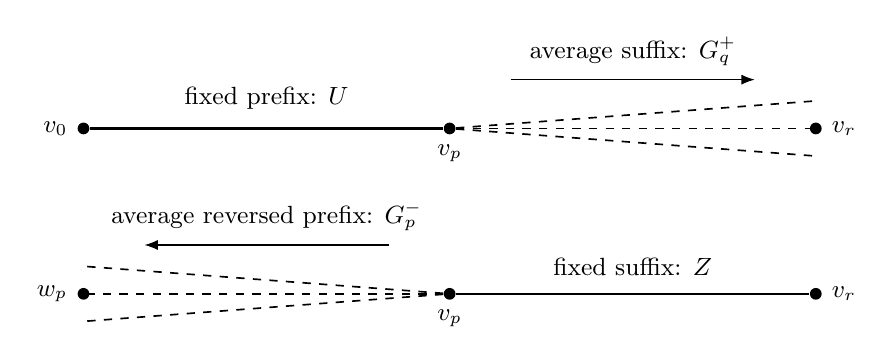
\begin{tikzpicture}[
  x=1.55cm,y=1cm,>=Latex,
  every node/.style={font=\small},
  vertex/.style={circle,fill,inner sep=1.5pt},
  fixed/.style={line width=.8pt},
  varied/.style={dashed,line width=.6pt}
]
  \node[vertex,label=left:{$v_0$}] (a) at (0,0) {};
  \node[vertex,label=below:{$v_p$}] (b) at (3,0) {};
  \node[vertex,label=right:{$v_r$}] (c) at (6,0) {};
  \draw[fixed] (a)--(b)
    node[midway,above=3pt] {fixed prefix: $U$};
  \foreach \h in {-.35,0,.35}
    \draw[varied] (b)--(6,\h);
  \draw[->] (3.5,.62)--(5.5,.62);
  \node at (4.5,.98) {average suffix: $G_q^+$};

  \node[vertex,label=left:{$w_p$}] (d) at (0,-2.1) {};
  \node[vertex,label=below:{$v_p$}] (e) at (3,-2.1) {};
  \node[vertex,label=right:{$v_r$}] (f) at (6,-2.1) {};
  \foreach \h in {-.35,0,.35}
    \draw[varied] (e)--(0,-2.1+\h);
  \draw[fixed] (e)--(f)
    node[midway,above=3pt] {fixed suffix: $Z$};
  \draw[->] (2.5,-1.48)--(.5,-1.48);
  \node at (1.5,-1.12) {average reversed prefix: $G_p^-$};
\end{tikzpicture}
\caption{The two averages in the half-path argument.
Solid halves are fixed and dashed halves are varied; each segment
represents a half-path, with one representative pair of endpoints labeled.
Arrows show the direction in which geometric extensions are enumerated.
In the lower row, the prefix is enumerated from $v_p$ toward
$w_p$, while its coefficients are traversed from $w_p$ to $v_p$,
giving the inward average $G_p^-$. The observation fields remain
unconditioned.}
\label{fig:half-path-averages}
\end{minipage}
\par\addvspace{\intextsep}


Suppose $r\ge2\ell_*(t)$.  Then $p,q\ge\ell_*(t)$.  Apply
\eqref{eq:dependent-average-bound} to the right side of
\eqref{eq:prefix-extension-average} with $\zeta=U^2$.  The
unconditional path variance bound and~\eqref{eq:path-discrepancy-bound}
give
$\E U^2\le C_{\mathrm{var}}pS$ and
$\|U^2\|_\infty\le p^2D_{\max,T}^2$.  Hence
\begin{equation}
 \E[P_r^2U^2]
 \le C_{\mathrm{cut}}C_{\mathrm{var}}
          e^{-\eta\omega(t)q}pS+D_{\max,T}^2p^2\varepsilon_q.
 \label{eq:weighted-prefix}
\end{equation}
Applying the same bound to~\eqref{eq:suffix-extension-average}, now
with $\zeta=Z^2$, gives
\begin{equation}
 \E[P_r^2Z^2]
 \le C_{\mathrm{cut}}C_{\mathrm{var}}
          e^{-\eta\omega(t)p}qS+D_{\max,T}^2q^2\varepsilon_p.
 \label{eq:weighted-suffix}
\end{equation}
These applications use the probability, under the joined law, of the
corresponding event determined by one observation marginal.  They do not
require a conditional variance bound or independence of that event
from the discrepancy.  The identical reasoning applies to $(P'_r)^2$
using the second marginal's path averages.

For $r\ge2$, both $p$ and $q$ are at least $r/3$.  Inserting the
four estimates into~\eqref{eq:path-half-split}, and using
$p+q=r$ and $p^2+q^2\le r^2$, proves the explicit inequality
\begin{equation}
 Q_r\le4C_{\mathrm{cut}}C_{\mathrm{var}}
             e^{-\eta\omega(t)r/3}rS
       +4D_{\max,T}^2r^2
             \exp\left(-\frac{b^{r/12}}{2b}\right).
 \label{eq:weighted-path-explicit}
\end{equation}

Finally fix $v_0$ and average the entire directed path over
$\mathcal P_r(v_0;\varnothing)$.  The stabilizer of $v_0$ is transitive on
these paths, and the vertex quantity $\Delta h_{v_0}$ is fixed in
every term.  Invariance gives the exact identity
\[
 L_r=\E[(\Delta h_{v_0})^2G_r^+(v_0;\varnothing)].
\]
For $r\ge\ell_*(t)$, use~\eqref{eq:dependent-average-bound} with
$\zeta=(\Delta h_{v_0})^2$, whose mean is $V$ and whose essential
supremum is at most $H_T^2$.  This yields
\begin{equation}
 L_r\le C_{\mathrm{cut}}e^{-\eta\omega(t)r}V
       +H_T^2\exp\left(-\frac{b^{r/4}}{2b}\right).
 \label{eq:weighted-root-explicit}
\end{equation}
Choosing one sufficiently small positive $c$ in the two explicit
bounds gives~\eqref{eq:weighted-paths}.  Finally,
$\ell_*(t)\le(C_0+1)/\omega(t)$ since $\omega(t)\le1$, which
proves the stated sufficient length condition.
\end{proof}

\section{Critical comparison and recovery}
\label{sec:uniqueness-factor}

We now show that two conditional copies with the same innovations agree
at the critical parameter $\theta=b^{-1/2}$, where $b=d-1\ge2$.
The weighted path estimates reduce the question to the variance
$V(t)=\E[(\Delta h_o(t))^2]$ of the site-field difference.
Their principal noise term has the scale
\[
 S(t)\sum_{r\ge1}r e^{-c\sqrt t\,r}\asymp \frac{S(t)}{t}
 \qquad(t\downarrow0),
\]
where $S(t)=\E[D_e(t)^2]$ and
$D_{(i,j)}=\log a(h_{j\to i})-\log a(h'_{j\to i})$.
The earlier estimate $S\le CV$ would leave a coefficient $1/t$,
which is not integrable at zero.  We improve it by using the fact that
$(\log a)'$ vanishes at the origin.  A field is usually small at early
times; the first result below makes the exceptional probability small
enough to compare it with any positive value of $V$.

\subsection{All moments and a small-field tail}

We use the fixed-time posterior identities and critical information
estimate already proved for one observation process.  At a deterministic
time $t>0$, fix an oriented edge $v\to w$ and write
\[
 Y=h_{v\to w}(t),\qquad M(t)=\E\tanh^2Y.
\]
The law of $Y$ is independent of the choice of edge and is symmetric.
Recall that $M(t)\le C\sqrt t$ for $0<t\le1$, that
$|Y-X_v(t)|\le b\beta$, and that
$X_v(t)=t\sigma_v+\sqrt t\,G$ with $G$ a standard normal variable
independent of the spin.  These are statements about the planted
observation law.  Each marginal of the conditional coupling has this
same law.

The second moment is critical because $b\theta^2=1$, whereas
$b\theta^p<1$ for every integer $p\ge3$; this strict contraction
lets the recursion propagate the second-moment scale to every higher
integer order.

\begin{lemma}[Critical field moments and tail]
\label{lem:critical-tail}
There are constants $0<K<\infty$ and $t_0\in(0,1)$, depending only on
$d$, such that for every integer $p\ge1$ and every $0<t\le t_0$,
\begin{equation}
 \E|h_{v\to w}(t)|^p\le e^{Kp^2}t^{p/4}.
 \label{eq:critical-all-moments}
\end{equation}
There are also $c>0$ and $t_{\mathrm{tail}}\in(0,t_0]$ such that
\begin{equation}
 \P\bigl(|h_{v\to w}(t)|>t^{1/8}\bigr)
 \le \exp\bigl(-c\log^2(1/t)\bigr),
 \qquad 0<t\le t_{\mathrm{tail}}.
 \label{eq:critical-field-tail}
\end{equation}
Both inequalities hold as well when conditioned on either value of the
component-root spin $\sigma_v$, or on either value of the deleted-neighbor
spin $\sigma_w$.
\end{lemma}

\begin{proof}
We begin with the second moment.  On $\{|X_v(t)|\le1\}$ the cavity
bound gives $|Y|\le1+b\beta$.  Comparison on this compact interval
therefore gives $Y^2\le C\tanh^2Y$.  On its complement we use
$Y^2\le2X_v(t)^2+2b^2\beta^2$.  For $t\le1/2$, the event
$|t\sigma_v+\sqrt t\,G|>1$ requires $|G|>1/(2\sqrt t)$.
Integration of the normal density, decreasing the positive exponent
constant if necessary, yields
\[
 \E\bigl[(1+X_v(t)^2)\mathbf 1_{\{|X_v(t)|>1\}}\bigr]
 \le C e^{-c/t}.
\]
Combining the two events with $M(t)\le C\sqrt t$ proves that, after
fixing some $t_0\le1/2$,
\begin{equation}
 A_2(t):=\E|Y|^2\le C\sqrt t,
 \qquad A_1(t):=\E|Y|\le C^{1/2}t^{1/4}
 \quad(0<t\le t_0).
 \label{eq:critical-moment-base}
\end{equation}
The second inequality is Cauchy--Schwarz.  The cavity bound also shows
that $A_p(t):=\E|Y|^p$ is finite for every integer $p\ge1$.

We next explain why the recursion can be expanded using independent
terms without changing these absolute moments.  For an integrable
function $f$, the spin-tilt identities from the posterior calculation
are
\begin{align*}
 \E[f(Y)\mid\sigma_v=\eta]
   &=\E[f(Y)(1+\eta\tanh Y)],\\
 \E[f(Y)\mid\sigma_w=\eta]
   &=\E[f(Y)(1+\eta\theta\tanh Y)],
 \qquad \eta\in\{-1,1\}.
\end{align*}
These are the identities \eqref{eq:component-field-tilts} from
Lemma~\ref{lem:component-spin-tilts}.
Because $Y$ has a symmetric marginal law, the term containing
$\tanh Y$ integrates to zero against every even function of $Y$.
In particular conditioning on either spin leaves each $A_p(t)$
unchanged.

Condition now on $\sigma_v=+1$ in the cavity recursion at $v$.
The own observation and the $b$ child-component observations are
independent under this conditional law: their spin transitions and
their planted noises lie in disjoint branches given the root spin.
The own observation has law $t+\sqrt t\,G$.  A child field is
conditioned through its deleted-neighbor spin, so the even-function
consequence of the second tilt gives, for every integer $r\ge1$,
\begin{equation}
 \E\bigl[|\psi(h_{u\to v}(t))|^r\mid\sigma_v=+1\bigr]
   =\E|\psi(Y)|^r\le\theta^r A_r(t).
 \label{eq:child-absolute-moments}
\end{equation}
Here $\psi(0)=0$ and $0<\psi'(z)\le\theta$ imply
$|\psi(z)|\le\theta|z|$.

There is an absolute constant $K_0$ such that
\begin{equation}
 \E|t+\sqrt t\,G|^r\le e^{K_0r^2}t^{r/4}
 \qquad(r\ge1\text{ an integer},\ 0<t\le1).
 \label{eq:own-gaussian-moments}
\end{equation}
Indeed, $|t+\sqrt t\,G|\le\sqrt t(1+|G|)$ in this time range,
and $\E|G|^r\le(C\sqrt r)^r$.  The inequality
$(x+y)^r\le2^{r-1}(x^r+y^r)$ for nonnegative $x,y$ bounds the
remaining constant by $e^{K_0r^2}$, uniformly over integer $r$.
We also used $t^{r/2}\le t^{r/4}$.

Choose $K\ge2K_0$ large enough that \eqref{eq:critical-all-moments}
holds for $p=1,2$, using \eqref{eq:critical-moment-base}.  Suppose it
holds for all positive integers below $p$, where $p\ge3$.
The triangle inequality in the cavity recursion, followed by the
multinomial expansion and the conditional independence just established,
bounds $A_p(t)$ by the expectation of the $p$th power of the sum of
the absolute values of the own term and the $b$ child terms.
The terms with exponent $p$ on a single child contribute at most
$b\theta^p A_p(t)$.  The term supported on the own observation is at
most $e^{Kp^2/2}t^{p/4}$ by \eqref{eq:own-gaussian-moments}.

Every other exponent vector $(r_0,r_1,\ldots,r_b)$ has sum $p$ and
at least two positive entries.  Hence every positive entry is below
$p$, and the induction hypothesis applies to its child factors.
Using \eqref{eq:own-gaussian-moments} for its own factor, if present,
and discarding powers of $\theta\le1$, its product of moments is at
most
\[
 e^{K\sum_{i=0}^b r_i^2}t^{p/4}.
\]
For such a vector,
$\sum_i r_i^2\le(p-1)^2+1=p^2-2(p-1)$: merging positive entries
until only two remain, then moving units to the larger one, can only
increase the sum of squares.  The sum of all multinomial coefficients
in $b+1$ slots is $(b+1)^p$.  Thus
\begin{equation}
 (1-b\theta^p)A_p(t)
 \le e^{Kp^2}t^{p/4}
   \left[e^{-Kp^2/2}+(b+1)^p e^{-2K(p-1)}\right].
 \label{eq:critical-moment-induction}
\end{equation}
The coefficient on the left is positive uniformly over $p\ge3$:
\[
 1-b\theta^p=1-b^{1-p/2}\ge\kappa_b:=1-b^{-1/2}>0.
\]
Enlarge the same constant $K$ once more so that
\[
 2K>\log(b+1),\qquad
 e^{-9K/2}+(b+1)^3e^{-4K}\le\kappa_b.
\]
Both terms in brackets in \eqref{eq:critical-moment-induction}
decrease as the integer $p$ increases from $3$.  Their sum is
therefore at most $\kappa_b\le1-b\theta^p$ for every such $p$.
Absorption proves \eqref{eq:critical-all-moments} with this single
$K$, for every integer order and all $t\le t_0$.

To obtain the tail, put $L=\log(1/t)$ and choose the integer
$p=\lfloor L/(16K)\rfloor$.  If $L\ge32K$, then
$L/(32K)\le p\le L/(16K)$.  Markov's inequality gives
\[
 \P(|Y|>t^{1/8})
 \le e^{Kp^2-pL/8}
 \le e^{-pL/16}
 \le e^{-L^2/(512K)}.
\]
Take $t_{\mathrm{tail}}\le\min(t_0,e^{-32K})$.
Both $|Y|^p$ and the indicator of the tail event are even functions
of $Y$, so the spin-tilt identities prove all the conditional
assertions as well.
\end{proof}

\subsection{Comparing log-factor and site-field differences}

Fix a finite horizon $T>0$.  The conditional-copy construction gives
\[
 |\Delta h_v(t)|\le H_T:=2T+2d\beta,
 \qquad 0\le V(t)\le H_T^2\quad(0\le t\le T),
\]
and Lemma~\ref{lem:copy-variance} makes $V$ absolutely continuous,
with $V(0)=0$.  Choose a constant, fixed throughout this horizon,
\begin{equation}
 K_T>\max\{1,H_T^2\},\qquad
 I(t)=1+\log\frac{K_T}{V(t)}\quad\text{when }V(t)>0.
 \label{eq:osgood-size}
\end{equation}
In particular $I(t)>1$, including at times when $V(t)\ge1$.

\begin{lemma}[Small-time log-factor estimate]
\label{lem:small-log-loss}
There is a fixed $t_*\in(0,\min\{t_{\mathrm{tail}},e^{-1}\}]$ such
that, for $0<t\le\min\{t_*,T\}$ with $V(t)>0$,
\begin{equation}
 S(t)\le C_T V(t)
   \left(t^{1/4}+\frac{I(t)}{\log^2(1/t)}\right).
 \label{eq:small-log-loss}
\end{equation}
At every time in $[0,T]$, the bound $S(t)\le CV(t)$ remains valid.
\end{lemma}

\begin{proof}
Write $Y=h_{j\to i}(t)$ and $Y'=h'_{j\to i}(t)$ for the edge used to
define $S(t)$.  The two cavity equations on this edge and
$|\psi'|\le\theta$ give the earlier comparison
\[
 |Y-Y'|\le\frac{|\Delta h_j|+\theta|\Delta h_i|}{1-\theta^2}.
\]
Invariance and Cauchy--Schwarz consequently give
\begin{equation}
 \E|Y-Y'|^2\le\frac{V(t)}{(1-\theta)^2},
 \qquad |Y-Y'|\le\frac{H_T}{1-\theta}.
 \label{eq:critical-component-comparison}
\end{equation}
Also
\[
 |(\log a)'(z)|
 =\frac{2(1-\theta^2)|\tanh z|}{1-\theta^2\tanh^2z}
 \le2|\tanh z|\le2.
\]
The global bound gives $S(t)\le4V(t)/(1-\theta)^2$ and
$|D_e(t)|\le2H_T/(1-\theta)$.

On the event $|Y|,|Y'|\le t^{1/8}$ the segment between them also lies
in that interval, and $|(\log a)'(z)|\le2t^{1/8}$ there.
The mean-value theorem and \eqref{eq:critical-component-comparison}
therefore give
\[
 \E[D_e(t)^2;\ |Y|,|Y'|\le t^{1/8}]
 \le\frac{4}{(1-\theta)^2}t^{1/4}V(t).
\]
For the complementary event the global square-integrable bound gives
$CV(t)$, while the deterministic bound on $D_e$ and a union bound
using \eqref{eq:critical-field-tail} in the two marginals give
$C_Te^{-c\log^2(1/t)}$.  Thus
\begin{equation}
 \E[D_e(t)^2;\ \max(|Y|,|Y'|)>t^{1/8}]
 \le\min\{CV(t),C_Te^{-c\log^2(1/t)}\}.
 \label{eq:bad-field-minimum}
\end{equation}
The argument uses only the two marginal probabilities; it requires
no independence between the two fields.

Set $u=V(t)>0$ and $J=\log^2(1/t)\ge1$.  If $u\le e^{-cJ/2}$,
then $I(t)\ge cJ/2$, so the first member of the minimum in
\eqref{eq:bad-field-minimum} is at most $C u I(t)/J$.
If $u>e^{-cJ/2}$, the second member divided by $u$ is at most
$C_Te^{-cJ/2}$.  Since $J e^{-cJ/2}$ is bounded for $J\ge1$
and $I(t)\ge1$, this is at most $C_T I(t)/J$.
Adding the small-field contribution proves \eqref{eq:small-log-loss}.
\end{proof}

\subsection{A cutoff depending on the discrepancy}

We next sum the weighted estimates.  Recall
$\omega(t)=\min\{\sqrt t,1\}$, and suppress $t$ at a fixed time
with $0<t\le T$ and $V(t)>0$.  The preceding path results give
\begin{align*}
 Q_r&\le C rS,\qquad L_r\le V &&(r\ge1),\\
 Q_r&\le C e^{-c\omega r}rS+C_T r^2e^{-\alpha b^{\gamma r}}
 &&(r\ge C_0'/\omega),\\
 L_r&\le C e^{-c\omega r}V+C_T e^{-\alpha b^{\gamma r}}
 &&(r\ge C_0'/\omega),
\end{align*}
for fixed positive constants $c,\alpha,\gamma,C_0'$ depending only on
$d$.  The last two lines follow from Proposition~\ref{prop:weighted-paths}, with
constants decreased or enlarged so that both exceptional terms have
the indicated common form.  These estimates include weights and
discrepancies formed from the same observations.

Choose $C_1$ sufficiently large that
\[
 C_1\ge C_0',\qquad \gamma C_1\log b\ge1,
 \qquad (\alpha/2)b^{\gamma C_1}\ge2,
\]
and take the integer
\begin{equation}
 R=\left\lceil C_1\bigl(\omega^{-1}+\log I\bigr)\right\rceil.
 \label{eq:variance-cutoff}
\end{equation}
The weighted estimates apply for $r>R$.  Since $\omega^{-1}\ge1$
and $I>1$, the choices above also give
\[
 (\alpha/2)b^{\gamma r}
 \ge (\alpha/2)b^{\gamma C_1\omega^{-1}}
                  I^{\gamma C_1\log b}
 \ge 2I \qquad(r>R).
\]
Splitting the exceptional exponent into equal halves therefore gives
\begin{equation}
 e^{-\alpha b^{\gamma r}}
 \le e^{-2I}e^{-(\alpha/2)b^{\gamma r}}
 =e^{-2}\left(\frac{V}{K_T}\right)^2
       e^{-(\alpha/2)b^{\gamma r}}
 \le V^2 e^{-(\alpha/2)b^{\gamma r}}\quad(r>R).
 \label{eq:exception-absorption}
\end{equation}
The last step uses $K_T>1$, and so remains valid when $V\ge1$.

\begin{lemma}[The noise and drift path sums]
\label{lem:cutoff-sums}
At each time $0<t\le T$ with $V(t)>0$,
\begin{equation}
 \begin{split}
 \sum_{r\ge1}Q_r
 &\le C_T\left[S\bigl(\omega^{-2}+(\log I)^2\bigr)+V^2\right],\\
 \sum_{r\ge1}\sqrt{Q_r}
 &\le C_T\left[\sqrt S\bigl(\omega^{-3/2}
                          +(\log I)^{3/2}\bigr)+V\right],\\
 \sum_{r\ge1}L_r
 &\le C_T\left[V\bigl(\omega^{-1}+\log I\bigr)+V^2\right].
 \end{split}
 \label{eq:cutoff-sums}
\end{equation}
\end{lemma}

\begin{proof}
For $r\le R$, the estimates $Q_r\le CrS$ and $L_r\le V$ give
the respective bounds
\[
 CS\sum_{r\le R}r\le CSR^2,
 \qquad C\sqrt S\sum_{r\le R}\sqrt r\le C\sqrt S R^{3/2},
 \qquad \sum_{r\le R}L_r\le VR.
\]
For the ordinary exponential terms at $r>R$, use
\begin{equation}
 \sum_{r\ge1}r^p e^{-c\omega r}
 \le C_{p,c}\omega^{-p-1}
 \quad\left(p\in\left\{0,\tfrac12,1\right\},\ 0<\omega\le1\right).
 \label{eq:exponential-length-sums}
\end{equation}
For example, compare the sum with
$\int_0^\infty(x+1)^p e^{-c\omega x}\,\mathrm dx$ and put
$y=\omega x$; since $\omega\le1$, the resulting integral is bounded
by $\omega^{-p-1}\int_0^\infty(y+1)^p e^{-cy}\,\mathrm dy$.
This gives $CS\omega^{-2}$ for the first sum and $CV\omega^{-1}$
for the third.  For the middle sum use
$\sqrt{x+y}\le\sqrt x+\sqrt y$; the ordinary exponential contribution
is bounded by $C\sqrt S\sum_{r\ge1}r^{1/2}e^{-c\omega r/2}
\le C\sqrt S\omega^{-3/2}$.

For the exceptional terms, \eqref{eq:exception-absorption} bounds
their three contributions by constants times
\[
 V^2\sum_{r\ge1}r^2e^{-(\alpha/2)b^{\gamma r}},\qquad
 V\sum_{r\ge1}r e^{-(\alpha/4)b^{\gamma r}},\qquad
 V^2\sum_{r\ge1}e^{-(\alpha/2)b^{\gamma r}},
\]
respectively.  Each series is finite because its exponential exponent
grows exponentially in $r$.  In the middle series the square root of
the $V^2$ factor is $V$, which is why the drift sum has this order.
Finally $\omega^{-1}+\log I\ge1$, so the ceiling in
\eqref{eq:variance-cutoff} gives
$R\le(C_1+1)(\omega^{-1}+\log I)$.
Bounding each power of this sum by a constant times the sum of its
corresponding powers proves \eqref{eq:cutoff-sums}.
\end{proof}

\subsection{An integrable comparison at time zero}

\begin{proposition}[Critical conditional-copy uniqueness]
\label{prop:critical-uniqueness}
For the invariant conditional coupling with common innovations at
$\theta=b^{-1/2}$, the site-field discrepancy satisfies
$V(t)=0$ for every $t\ge0$.
\end{proposition}

\begin{proof}
Work on the fixed horizon $[0,T]$ used above.  Inserting the noise
and drift bounds \eqref{eq:noise-bound} and~\eqref{eq:drift-bound}
into the variance identity~\eqref{eq:variance}, and using
$n_r\theta^{2r}=db^{r-1}b^{-r}=d/b$ for $r\ge1$, gives
\begin{equation}
 V'(t)\le C\left(
 V(t)+\sum_{r\ge1}Q_r(t)+\sum_{r\ge1}L_r(t)
            +\sqrt{V(t)}\sum_{r\ge1}\sqrt{Q_r(t)}\right)
 \label{eq:variance-path-reduction}
\end{equation}
for almost every $t$.  The sums in Lemma~\ref{lem:cutoff-sums} are
finite at the positive times with $V(t)>0$ where we now use this
inequality.

Insert those three bounds into \eqref{eq:variance-path-reduction}.
Use $S\le CV$, and hence $\sqrt{VS}\le C V$, for all terms except
$S\omega^{-2}$.  The bounds $V\le H_T^2$ imply
$V^{3/2}\le H_TV$ and $V^2\le H_T^2V$.  Finally
\[
 (\log I)^p\le C_p I\qquad(I\ge1,\ 0<p\le2),
\]
since $x^p e^{-x}$ is bounded on $x\ge0$.  As $\omega^{-1}\le
\omega^{-3/2}$, all the terms just treated are at most
\[
 C_TV\bigl(I+\omega^{-3/2}\bigr).
\]
This identifies the worst drift contribution explicitly:
$\sqrt{VS}\,\omega^{-3/2}\le CV\omega^{-3/2}$.

For $0<t\le\min\{t_*,T\}$, we have $\omega=\sqrt t$.
Lemma~\ref{lem:small-log-loss} gives the remaining estimate
\[
 S\omega^{-2}
 \le C_TV\left(t^{-3/4}
           +\frac{I}{t\log^2(1/t)}\right).
\]
Together with $I\ge1$, the preceding bounds prove
\begin{equation}
 V'(t)\le k_T(t)V(t)
        \left(1+\log\frac{K_T}{V(t)}\right)
 \quad\text{for almost every $t\in(0,T]$ with $V(t)>0$},
 \label{eq:integrable-osgood}
\end{equation}
where, after increasing $C_T$, we may take
\begin{equation}
 k_T(t)=
 \begin{cases}
 C_T\left(1+t^{-3/4}
          +\dfrac{1}{t\log^2(1/t)}\right),&0<t\le\min\{t_*,T\},\\[2mm]
 C_T,&t_*<t\le T.
 \end{cases}
 \label{eq:osgood-coefficient}
\end{equation}
For the second branch, $\omega(t)\ge\sqrt{t_*}>0$ because
$t_*\le1$; there we use $S\le CV$ also for $S\omega^{-2}$.
Thus that branch is bounded on the whole later interval.
If $T\le t_*$ there is no later interval.  The small-time expression
is used only for $t\le t_*\le e^{-1}$, and it is integrable there:
\[
 \int_0^{t_*}t^{-3/4}\,\mathrm dt=4t_*^{1/4},\qquad
 \int_0^{t_*}\frac{\mathrm dt}{t\log^2(1/t)}
 =\frac{1}{\log(1/t_*)}.
\]
In particular $k_T\in L^1(0,T)$.

We finish with an Osgood-type comparison~\cite{Osgood1898}, proving
the needed absolutely continuous form directly.  Suppose that $V$ is positive somewhere
on $[0,T]$.  Choose such a time $t$, and let $a<t$ be the left
endpoint of its component in the positivity set of $V$.
Continuity and $V(0)=0$ give $V(a)=0$.  On any closed interval
$[u,t]$ with $a<u<t$, continuity bounds $V$ away from zero.
The function $z\mapsto\log(1+\log(K_T/z))$ has bounded derivative
on the range of $V$ on that interval.  Its composition with the
absolutely continuous function $V$ is therefore absolutely continuous,
and the chain rule and \eqref{eq:integrable-osgood} give
\[
 (\log I)'=-\frac{V'}{VI}\ge-k_T\quad\text{almost everywhere on }[u,t].
\]
Integrating yields
\[
 \log I(u)\le\log I(t)+\int_u^t k_T(s)\,\mathrm ds
             \le\log I(t)+\int_a^t k_T(s)\,\mathrm ds<\infty.
\]
The last bound is independent of $u$.  But $V(u)\to V(a)=0$ as
$u\downarrow a$, so $I(u)\to\infty$ and $\log I(u)\to\infty$,
a contradiction.  Hence $V$ vanishes on $[0,T]$.  Since the horizon
was arbitrary, it vanishes at every time.
\end{proof}

\subsection{Recovering the observations and the spin factor}
\label{sec:recovery}

The comparison has now proved $V(t)=0$ for the particular copies
sampled in~\eqref{eq:copy-law}: Proposition~\ref{prop:strict-uniqueness}
handles $b\theta^2<1$, and Proposition~\ref{prop:critical-uniqueness}
handles $b\theta^2=1$. We first deduce equality of their observation
paths and turn it into a Borel map from innovations to observations.
The spins will then be read from the integer-time slopes of those paths.

The final passage to a spin map equivariant on every input uses local
conditional expectations.

\begin{lemma}[Pointwise equivariance of spin factors]
\label{lem:pointwise-spin-factor}
Let $(U_v)_{v\in\mathcal V}$ be independent uniform labels on $T_d$.
Suppose a Borel map
$\Phi:[0,1]^{\mathcal V}\to\{-1,1\}^{\mathcal V}$ satisfies
$\Phi(gU)=g\Phi(U)$ almost surely for each fixed
$g\in\Aut(T_d)$. There is a Borel map
$\Psi:[0,1]^{\mathcal V}\to\{-1,1\}^{\mathcal V}$ such that
$\Psi(U)=\Phi(U)$ almost surely and
\[
 \Psi(gx)=g\Psi(x)
 \qquad\text{for every }x\in[0,1]^{\mathcal V}
                 \text{ and }g\in\Aut(T_d).
\]
\end{lemma}

\begin{proof}
Fix an auxiliary vertex $o$. For each integer $R\ge0$, choose a
Borel function $h_R:[0,1]^{B_R(o)}\to[-1,1]$ representing
\[
 \E[\Phi(U)_o\mid U|_{B_R(o)}].
\]
A Borel version exists, and clipping it to $[-1,1]$ preserves this
conditional expectation. Let $G_R$ be the finite automorphism group
of the rooted ball $B_R(o)$, and average:
\[
 q_R(y)=\frac1{|G_R|}\sum_{a\in G_R}h_R(ay).
\]
Every $a\in G_R$ extends to a tree automorphism fixing $o$: outside
the ball, match the isomorphic rooted components attached to its
boundary. Such an extension preserves the IID law and the ball's
label sigma-field. The assumed almost-sure equivariance therefore
makes $h_R(a(U|_{B_R(o)}))$ another version of the same conditional
expectation. Thus $q_R$ still represents that conditional expectation,
and is Borel, bounded by one, and invariant under $G_R$ on every input.

Apply this same local rule at every vertex. Explicitly, for a rooted
isomorphism $\iota:B_R(o)\to B_R(v)$, put
\[
 A_R(x)_v=q_R\bigl((x_{\iota(u)})_{u\in B_R(o)}\bigr).
\]
Two choices of $\iota$ differ by an element of $G_R$, so the value
does not depend on this choice. The maps $A_R$ are consequently
Borel and satisfy $A_R(gx)=gA_R(x)$ for every input and automorphism.
Each $\iota$ also extends to a tree automorphism taking $o$ to $v$.
Transporting the conditional expectation by this fixed automorphism
shows that
\[
 A_R(U)_v=\E[\Phi(U)_v\mid U|_{B_R(v)}]
                  \quad\text{almost surely}.
\]
The ball sigma-fields increase to the full label sigma-field.
Upward martingale convergence, together with a countable intersection
over vertices and radii, gives $A_R(U)_v\to\Phi(U)_v$ simultaneously
at every vertex almost surely.

On every label input define
\[
 \Psi(x)_v=
 \begin{cases}
  1,&\limsup_{R\to\infty} A_R(x)_v\ge0,\\
 -1,&\limsup_{R\to\infty} A_R(x)_v<0.
 \end{cases}
\]
Boundedness makes each limsup finite, and this formula defines a
Borel spin map. The pointwise equivariance of every $A_R$ passes
through the limsup and the common threshold. On the simultaneous
convergence event the limits belong to $\{-1,1\}$, so
$\Psi(U)=\Phi(U)$ almost surely.
\end{proof}

\begin{proposition}[Recovery of observations and spins]
\label{prop:factor-extraction}
Fix $d\ge3$ and $0<\theta=\tanh\beta\le(d-1)^{-1/2}$, and retain
the path spaces and laws $\mathsf Q,\mathsf w,\mathsf K$ defined in
Section~\ref{sec:coupling}. There is a Borel map
$F:\mathsf W\to\mathsf X$ such that
\[
 \mathsf K(w,\cdot)=\delta_{F(w)}
       \quad\text{for $\mathsf w$-almost every }w,
 \qquad X=F(W)\quad\mathsf Q\text{-almost surely}.
\]
For each fixed $g\in\Aut(T_d)$,
$F(gW)=gF(W)$ almost surely. The free Ising law is the law of a
Borel map of vertex IID uniform labels which commutes with every
automorphism on every label input. The same spin-factor
conclusion holds at $\theta=0$.
\end{proposition}

\begin{proof}
First suppose $\theta>0$. The two uniqueness propositions give
$V(t)=0$ for every deterministic time in their respective parameter
ranges. Invariance permits any vertex in place of the auxiliary
vertex $o$. Intersecting the full-probability events for all vertices
and nonnegative rational times gives
$h_v(q)=h'_v(q)$ simultaneously at those indices. Both field arrays
are continuous, so they agree at every time and vertex. Hence their
magnetizations agree, and the common innovation identity gives
\[
 X_v(t)=W_v(t)+\int_0^t m_v(s)\dd s
       =W_v(t)+\int_0^t m'_v(s)\dd s=X'_v(t).
\]
Thus $\widehat{\mathsf Q}\{X=X'\}=1$ as an equality of full path
configurations. The use of rational times avoided an uncountable
intersection over time.

For $v\in\mathcal V$ and $q\in\mathbb Q_{\ge0}$ choose the finite
Borel version
\[
 f_{v,q}(w)=\int x_v(q)\,\mathsf K(w,\dd x)
\]
when the absolute integral is finite, and set it to zero otherwise.
Kernel integration makes this Borel, and integrability of $X_v(q)$
ensures that the exceptional inputs have $\mathsf w$-measure zero.
Taking expectations in~\eqref{eq:copy-coordinate-variance} and using
$X=X'$ gives
\[
 0=\E_{\widehat{\mathsf Q}}(X_v(q)-X'_v(q))^2
   =2\E_{\mathsf Q}\Var(X_v(q)\mid W).
\]
It follows that $X_v(q)=f_{v,q}(W)$ almost surely. We may impose
these identities simultaneously for all the countably many pairs
$(v,q)$. Disintegrating them shows that, for $\mathsf w$-almost
every $w$, $\mathsf K(w,\cdot)$ gives mass one to
\[
 \{x\in\mathsf X:x_v(q)=f_{v,q}(w)
                 \text{ for every }v,q\}.
\]
This set has at most one element, since continuous paths are
determined by their rational-time values. Its conditional mass one
also makes it nonempty. Thus $\mathsf K(w,\cdot)$ is a point mass
for almost every $w$.

The conditional point-mass principle for measurable recovery also
appears in Kurtz~\cite[Lemma~1.3 in arXiv:1305.6747v2]{Kurtz2014}.
We give a Borel choice of that path, including values on all other
inputs. For each $v$ and integer $j\ge1$, let $p_{v,j}(w)$ be the
piecewise linear path whose value at $k2^{-j}$ is
$f_{v,k2^{-j}}(w)$ for every integer $k\ge0$. These are Borel maps
to $C([0,\infty),\mathbb R)$ with its locally uniform topology.
Let $\mathcal G$ be the set of $w$ for which, at every vertex, these
paths are Cauchy uniformly on every compact interval and
$f_{v,0}(w)=0$. This set is Borel. Indeed, the uniform Cauchy
condition on $[0,N]$ can be tested by the supremum over rational
times there, and the quantifiers over vertices, integers $N$, error
levels, and pairs of sequence indices are all countable. On
$\mathcal G$ the limits are continuous paths starting at zero.
Define $F_v(w)$ to be this limit for $w\in\mathcal G$, and let
$F(w)$ be the all-zero path configuration for $w\notin\mathcal G$.
The limit map on the Cauchy set of a Polish space is Borel, so this
defines a Borel map $F:\mathsf W\to\mathsf X$.

For almost every $w$, the rational coordinates just specified are
those of the unique path configuration charged by $\mathsf K(w,\cdot)$.
Uniform continuity of each such path on compact intervals shows
that its dyadic linear interpolants converge uniformly there.
Consequently $w\in\mathcal G$ and $F(w)$ is that configuration.
This proves both $\mathsf K(w,\cdot)=\delta_{F(w)}$ almost everywhere
and $X=F(W)$ in the original law.

Fix now one automorphism $g$. Invariance of $\mathsf Q$ and
uniqueness of conditional expectations imply
\begin{equation}\label{eq:recovery-coordinate-equivariance}
 f_{v,q}(gw)=f_{g^{-1}v,q}(w)
       \quad\text{for $\mathsf w$-almost every }w
\end{equation}
for each $v,q$. Intersecting over those countably many pairs gives
all these identities simultaneously for this fixed $g$. The dyadic
interpolants then obey
$p_{v,j}(gw)=p_{g^{-1}v,j}(w)$ for every $v,j$. On this full-measure
set, $w\in\mathcal G$ if and only if $gw\in\mathcal G$, because
its defining Cauchy conditions are the same after permuting vertices.
The all-zero default is invariant as well, so
$F(gw)=gF(w)$ almost surely. The full-measure set in this argument
is allowed to depend on $g$; none is asserted for all automorphisms
at once.

Define a spin map on every innovation input by
\begin{equation}\label{eq:spin-factor}
 H_v(w)=
 \begin{cases}
 \displaystyle\lim_{n\to\infty}\frac{F_v(w)(n)}{n},
   &\text{if this limit exists and belongs to $\{-1,1\}$},\\[2mm]
 1,&\text{otherwise}.
 \end{cases}
\end{equation}
Existence of either indicated limit is a Borel condition expressed
through countably many error bounds and integer indices. Thus each
$H_v$ is Borel, and so is $H$ into the countable spin product.
On the planted probability space,
\[
 \frac{F_v(W)(n)}n=\frac{X_v(n)}n
      =\sigma_v+\frac{B_v(n)}n
\]
simultaneously for the integer indices. For every $\varepsilon>0$,
the Gaussian tail bound gives
\[
 \sum_{n\ge1}\P(|B_v(n)|>\varepsilon n)
       \le\sum_{n\ge1}2e^{-\varepsilon^2n/2}<\infty.
\]
Borel--Cantelli, first for positive rational $\varepsilon$ and then
over the countable vertex set, gives $B_v(n)/n\to0$ simultaneously
for every vertex. Therefore $H(W)=\sigma$ almost surely. Under
product Wiener input, $H$ has exactly the free zero-field Ising law.
For the fixed $g$ above, the identity $F(gw)=gF(w)$ makes the
sequences in~\eqref{eq:spin-factor} agree after the same permutation.
Their limits and their failure cases consequently agree. The same
default sign at every site gives $H(gw)=gH(w)$ almost surely.

Finally, Wiener measure is a Borel probability measure on the Polish
space $C_0([0,\infty),\mathbb R)$. The standard Borel sampling
theorem therefore supplies a Borel map
$\xi:[0,1]\to C_0([0,\infty),\mathbb R)$ which sends Lebesgue measure
to Wiener measure. For independent uniform labels $(U_v)$, set
\[
 \Phi(U)=H\bigl((\xi(U_v))_{v\in\mathcal V}\bigr).
\]
Applying the same $\xi$ at every site gives product Wiener law and
commutes pointwise with every vertex permutation. Thus $\Phi$ is
Borel, has law $\mu_{d,\beta}$, and satisfies
$\Phi(gU)=g\Phi(U)$ almost surely for each fixed $g$.
Lemma~\ref{lem:pointwise-spin-factor} replaces $\Phi$ by a Borel map
with the same law that is equivariant on every label input.

When $\theta=0$, the broadcast law is already a product of fair signs.
The rule $\Phi_v(U)=1$ for $U_v\le1/2$ and $\Phi_v(U)=-1$ otherwise
gives that law and commutes with every permutation for every input.
All choices above are for the fixed pair $(d,\beta)$. Together with
the known converse in Section~\ref{sec:introduction}, this proves
Theorem~\ref{thm:main}.
\end{proof}

\bibliographystyle{plainnat}
\bibliography{references/references}
\end{document}
